%%
%% licence       kaneton licence
%%
%% project       kaneton
%%
%% file          /home/mycure/kaneton/view/papers/kaneton/kaneton.tex
%%
%% created       julien quintard   [thu dec  8 00:26:00 2005]
%% updated       julien quintard   [fri mar 10 02:20:09 2006]
%%

%
% template
%

%
% ---------- header -----------------------------------------------------------
%
% project       kaneton
%
% license       kaneton
%
% file          /home/mycure/kaneton/view/template/book.tex
%
% created       julien quintard   [wed may 16 18:16:50 2007]
% updated       julien quintard   [sun jun  3 12:00:37 2007]
%

%
% class
%

\documentclass[10pt,a4wide]{book}

%
% packages
%

\usepackage[english]{babel}
\usepackage[T1]{fontenc}
\usepackage{a4wide}
\usepackage{fancyheadings}
\usepackage{multicol}
\usepackage{indentfirst}
\usepackage{graphicx}
\usepackage{color}
\usepackage{xcolor}
\usepackage{verbatim}

\usepackage{aeguill}

\usepackage[Lenny]{\path/package/fncychap}

\pagestyle{fancy}

%
% -
%

\renewcommand{\-}{\vspace{\parskip}}

%
% toc
%

\newcommand{\toc}
  {
    \tableofcontents
    \setlength{\footrulewidth}{0.3pt}
    \setlength{\parindent}{0.3cm}
    \setlength{\parskip}{2ex plus 0.5ex minus 0.2ex}
  }

%
% logos
%

\newcommand{\logos}
  {
    \begin{center}
      
\includegraphics[scale=0.8]{\path/logo/kaneton.pdf}
    \end{center}
  }

%
% colors
%

\definecolor{functioncolor}{rgb}{0.40,0.00,0.00}
\definecolor{commandcolor}{rgb}{0.00,0.00,0.40}
\definecolor{verbatimcolor}{rgb}{0.00,0.40,0.00}
\definecolor{noticecolor}{rgb}{0.87,0.84,0.02}

%
% function
%

\newcommand\function[3]{
  \begin{tabular}{p{0.2cm}p{13.8cm}}
  & {\color{functioncolor}\textbf{#1}}#2
  \end{tabular}

  \begin{tabular}{p{1cm}p{13cm}}
  & #3
  \end{tabular}}

%
% align
%

\newcommand\align[1]{
  \\ & \hspace{#1}}

%
% argument
%

\newcommand\argument[1]{\textit{#1}}

%
% command
%

\newcommand\command[2]{
  \begin{tabular}{p{0.2cm}p{13.8cm}}
  & {\color{commandcolor}\textbf{#1}}
  \end{tabular}

  \begin{tabular}{p{1cm}p{13cm}}
  & #2
  \end{tabular}}

%
% notice
%

\newcommand\notice[1]{
  {\color{noticecolor}\textbf{Notice}}

  \begin{tabular}{p{0.2cm}p{13.8cm}}
  & #1
  \end{tabular}}

%
% subsubsubsection
%

\newcommand\subsubsubsection[1]{\textbf{#1}}

%
% example
%

\newcommand\example[1]{
  \textit{Example:}

  \begin{tabular}{p{0.2cm}p{13.8cm}}
  & \textit{#1}
  \end{tabular}}

%
% warning XXX
%

\renewcommand{\familydefault}{\sfdefault}

%
% verbatim stuff
%

\makeatletter

\renewcommand{\verbatim@font}
  {\ttfamily\footnotesize\selectfont}

\def\verbatim@processline{
  \hskip15ex{\color{verbatimcolor}\the\verbatim@line}\par
}

\makeatother

%
% header
%

\rhead{}
\rfoot{\scriptsize{The kaneton microkernel project}}

\date{\scriptsize{\today}}


%
% header
%

\lhead{\scriptsize{The kaneton microkernel project reference}}
\rhead{}

%
% title
%

\title{The kaneton microkernel reference
       \logos}

%
% authors
%

\author{\small{Julien Quintard},
        \small{Matthieu Bucchianeri},
        \small{Renaud Voltz}}

%
% document
%

\begin{document}

%
% title
%

\maketitle

%
% --------- text --------------------------------------------------------------
%

%
% authors
%

This document describes the kaneton microkernel reference project.

This document should be used by every student willing implement the
kaneton microkernel as people looking for more details on the kaneton
microkernel design and implementation.

All the kaneton documents are available on
the official website
  \footnote{http://www.kaneton.org}.

%
% toc
%

\tableofcontents

%
% chapters
%

%%
%% licence       kaneton licence
%%
%% project       kaneton
%%
%% file          /home/mycure/kaneton/view/papers/kaneton/goals.tex
%%
%% created       matthieu bucchianeri   [mon jan 30 17:09:17 2006]
%% updated       julien quintard   [thu mar  2 01:21:16 2006]
%%

%
% goals
%

\chapter{Goals}

The kaneton microkernel is studied during the EPITA System, Network
and  Security specialization. The project comes with many courses
leading student to learn about architectures and kernels and to design
and develop important parts of a microkernel.

From this fact, kaneton has been designed in a very particular way to
keep the design as simple as possible to be understandable by the
students.

kaneton is not based on any previous kernel code: it is written from
scratch. As we wanted the kernel to be portable on any architecture,
we paid particular attention in dividing the code into two precise
sections: the architecture-independent code and the
architecture-dependent code.

---

We also use terms to design these two different pieces of code, the
\textbf{core} and the \textbf{arch} respectively. These terms are not
quite defined and are not very clear and expressive but we chose them.

---

Designing this portability system, we intended to port the kernel on
many architectures, so we had to keep the architecture-dependent code
as small as possible. Moreover, the only requirement about the
hardware is the minimal amount of memory, which must be at least 32
megabytes.

As we wanted the project to be very pedagogic, kaneton source code is
clear and heavily commented. Each manager has its own directory and
headers. Function names and prototypes are unified and explicit.
Each function is preceded by a header explaining the task it performs
and detailing the different steps.

%
% history
%

\section{History}

%
% year 2006
%

\subsection{Year 2006}

The kaneton project comes with a development environment. Then the
students have to write parts of the microkernel without having to
build a development environment from scratch which takes much time.

Moreover, courses were added to the EPITA specialization curriculum
including microprocessor's architectures, kernels history etc..

%
% year 2005
%

\subsection{Year 2005}

The first complete kaneton project was scheduled from January to December.

%
% year 2004
%

\subsection{Year 2004}

The project was introduced by students willing learn kernel architectures.

%%
%% licence       kaneton licence
%%
%% project       kaneton
%%
%% file          /home/mycure/kaneton/view/papers/kaneton/history.tex
%%
%% created       julien quintard   [sat mar  4 14:15:39 2006]
%% updated       julien quintard   [mon may  8 17:48:32 2006]
%%

%
% history
%

\chapter{History}

In this chapter we will detail the kaneton history from the first
year with low-level programming introduction to the last kaneton
reference implementation.

\newpage

%
% text
%

\textit{Since this chapter is intended to retrace the kaneton history,
  no insurance can be made on emails validity.}

As said in the previous chapter, the kaneton microkernel was introduced
by two students
Julien Quintard
  \footnote{julien.quintard@gmail.com} and
Jean-Pascal Billaud
  \footnote{billau\_j@epita.fr}
during the year 2004.

The kaneton microkernel is currently studied during the
EPITA
  \footnote{http://www.epita.fr}
System, Network and Security specialization curriculum
  \footnote{http://srs.epita.fr}.

During the kaneton history, the project evolved and lectures were added
to the curriculum to make the whole kaneton project more interesting and
understandable by the students.

%
% year 2004
%

\section{Year 2004}

The first year, a low-level programming introduction course was proposed
for the engineering school's first year students.

Then, about fourteen hours courses were made to introduce microprocessor's
external architecture and low-level programming.

The students had to develop small, poor and messy device drivers for the
console and keyboard peripherals. Moreover, a tiny shell was developed
by students so they were able to enter a command to launch a special
kernel action.

The course was a bit chaotic but this first shot was a success.

Therefore, the System, Network and Security specialization students
themselves asked the two students a more evolved project in their
curriculum so they were able to learn about operating systems internals.

%
% year 2005
%

\section{Year 2005}

Then, for the next year, the two students prepared a complete microkernel
design with two complete courses on kernel design and Intel Architecture
programming.

Moreover, other students joined the project:
C\'edric Aubouy
  \footnote{aubouy\_c@epita.fr},
Fabien Le-Mentec
  \footnote{le-men\_f@epitech.net} and
Renaud Lienhart
  \footnote{lienha\_r@epita.fr}.

The project was composed of six steps, from the bootstrap, passing by
the kernel internals including memory management, task management etc..
to the servers with an IDE device driver and finally a FAT file system.

Once again, the whole project was a success but the kaneton people
noticed that the students took much time doing boring work like
filling in header files, dealing with versionning problems, writing
makefiles and shell scripts etc..

Moreover, the courses were too messy and the students had difficulties
to make the relation between kaneton design and microprocessor's
architecture implementation.

Finally, kaneton people started to implement a kaneton microkernel
reference in C language.

%
% year 2006
%

\section{Year 2006}

People joined the project:
Matthieu Bucchianeri
  \footnote{bucchi\_m@epita.fr} and
Renaud Voltz
  \footnote{voltz\_r@epita.fr}.

These students actively contributed to the kaneton implementation.

This year, kaneton people decided to introduce a development environment,
based on the kaneton implementation reference, including everything
necessary to set up a collaborative kernel development.

While, previously, the students had to write the entire microkernel
and servers from scratch, this year, students only had to write precise
parts of the microkernel.

These major modifications in the kaneton project were made to
allow students to explore advanced fields like distributed systems
aspects and/or microkernel's security.

Finally, courses were added to the EPITA System, Network and Security
specialization curriculum including microprocessor's architectures,
kernels history etc..

The kaneton microkernel implementation, in 2006, counted about
\textit{7,000} lines for the core and about \textit{2,000} lines for the
microprocessor's architecture implementation.

Nevertheless, the microkernel is not complete yet, so a full implementation
of about \textit{15,000} lines can be expected which seems correct
considering the kaneton microkernel advanced design.

%%
%% licence       kaneton licence
%%
%% project       kaneton
%%
%% file          /home/mycure/kaneton/view/papers/kaneton/overview.tex
%%
%% created       matthieu bucchianeri   [mon jan 30 17:09:45 2006]
%% updated       julien quintard   [thu mar  2 13:12:22 2006]
%%

%
% overview
%

\chapter{Overview}

XXX ce chapitre va vous aider a reconnaitre les fonctionnalites principale
XXX d'un kernel dans kaneton.

The kaneton microkernel is only the core of an operating system.
Main tasks like hardware drivers or user services are implemented as
\textbf{servers}. So the microkernel only has a few functionalities to
provide:

\begin{itemize}
  \item
    Memory management.
  \item
    Process management.
  \item
    Communication.
  \item
    Events.
\end{itemize}

In this chapter we will describe briefly these tasks and all the
associated managers.

%
% memory management
%

\section{Memory Management}

Handling the memory -- from virtual address space to physical
addressing -- is done by three major managers, the \textbf{as},
\textbf{segment} and \textbf{region} managers.

%
% as
%

\subsection{as}

The address space manager just manages the different address spaces
used by the kaneton tasks.

In kaneton, we call an \textbf{as - address space} a list of memory
locations referenced by a task. Each task has its own address space.

%
% segment
%

\subsection{segment}

The segment manager just manages the segments reserved by
the different kaneton entities including the kernel, the drivers etc..

In kaneton terms a \textbf{segment} is a contiguous area of reserved
physical memory.

%
% region
%

\subsection{region}

The region manager keeps track of regions used to map segments for
each address space reserved on the system.

In kaneton, a \textbf{region} is contiguous area of virtual memory
mapping a segment's part.

%
% process management
%

\section{Process Management}

XXX

%
% communication
%

\section{Communication}

XXX

%
% events
%

\section{Events}

XXX

%
% ---------- header -----------------------------------------------------------
%
% project       kaneton
%
% license       kaneton
%
% file          /home/mycure/kaneton/view/book/development/source-tree.tex
%
% created       julien quintard   [thu may 17 22:41:36 2007]
% updated       julien quintard   [sun may 20 18:09:37 2007]
%

%
% ---------- source tree ------------------------------------------------------
%

\chapter{Source Tree}

In this chapter we will briefly describe the kaneton microkernel project
source tree.

\newpage

%
% ---------- text -------------------------------------------------------------
%

The kaneton microkernel reference source tree looks like the following
listing:

\begin{verbatim}
cheat/
environment/
export/
configure/
kaneton/
library/
license/
tool/
test/
transcript/
view/
\end{verbatim}

% cheat/

\subsection*{cheat/}

Since the kaneton microkernel is implemented by students, the kaneton
people need to check whether students are cheating by re-using parts of
previous years projects or other kernel source code available on the
\textit{Internet}.

To avoid cheating, kaneton people developed a software checking for
commonalities between different source codes.

The \textit{cheat/} kaneton subdirectory contains everything necessary
to perform such tasks including the software, the different source codes
found on the internet, the kaneton students' implementation from the
previous years etc.

% environment/

\subsection*{environment/}

This directory contains everything necessary to the kaneton development
environment.

The kaneton development environment allows different developers to
interact on the development of the same microkernel in a pretty easy way.

The development environment aims at providing developers to possibility to
work in a collaborative manner without interfering with each other. These
developers are likely to run different operating systems on different
microprocessors. In addition, the kaneton microkernel can be targeted for
different microprocessor architectures. The development environment was
introduced to cope with these combinaisons by providing profiles, each
profile describing the behaviour of a component: underlying operating system,
target architecture, user-specific stuff etc.

As a result, each developer can use a different operating system and
microprocessor architecture with his own specific compiling flags, kaneton
parameters etc. without modifying another developer's configuration.

% export/

\subsection*{export/}

The \textit{export/} directory contains scripts used to generate a kaneton
tarball in order to be distributed to the students at the beginning of the
kaneton project.

Indeed, these scripts rearrange the kaneton hierarchy hidding some
important directories the students do not need to be aware of.

Moreover some source code parts are removed since the students then have to
rewrite these piece of code.

% configure/

\subsection*{configure/}

This directory contains everything necessary for configuring its own
kaneton microkernel development environment through the compiling process
to the boot system.

Any new contributor should first look at this directory.

% kaneton/

\subsection*{kaneton/}

This directory is the most important of the project since it contains
the whole microkernel source code.

The directory is composed of three important subdirectories: \textit{core/},
\textit{platform} and \textit{architecture}. These subdirectories are described
next.

% kaneton/core/

\subsection*{kaneton/core/}

This directory contains the kaneton core source code.

The directory is divided as shown below:

\begin{verbatim}
as/
region/
sched/
segment/
set/
task/
thread/
[...]
\end{verbatim}

Each directory represents a kaneton core manager. For more information on
the kaneton core, please refer to the appropriate document:
\textit{The kaneton microkernel :: reference implementation}

% kaneton/platform/

\subsection*{kaneton/platform/}

This directory contains everything in relation with what the kaneton
microkernel project calls a \textbf{platform}. The platform represents the
board supporting the devices: microprocessor, memory, peripherals etc.

This directory obviously contains subdirectories for each platform
supported by the kaneton microkernel.

% kaneton/architecture

\subsection*{kaneton/architecture}

The \textit{architecture} directory contains the source-code related to
the microprocessor architecture.

This directory is composed of subdirectories, each one representing an
architecture: \textit{ia32}, \textit{mips64} etc.

% library/

\subsection*{library/}

This directory contains the libraries used either by the kaneton microkernel
itself or by the kaneton microkernel servers. This directory especially
contrains the standard \textit{kaneton C library}.

% license/

\subsection*{license/}

This directory contains the licenses used for any program or document
in relation with the kaneton microkernel project.

Each student has to read and accept the kaneton license before implementing
or even using the kaneton microkernel project.

% tool/

\subsection*{tool/}

This directory contains additional files used by the kaneton development
environment.

% test/

\subsection*{test/}

Since the kaneton microkernel is used as a material for operating system
courses, the kaneton microkernel reference which is the basis of students'
work is to be extremely reliable.

The kaneton project therefore contains a set of tools in order to validate
the kaneton reference implementation behaviour. These tools are also used
for evaluating the correctness of the students' implementation.

The \textit{test/} directory so contains the set kaneton scripts and tests
for validating a kaneton microkernel implementation.

% transcript/

\subsection*{transcript/}

This directory contains real-time recorded sessions. These sessions can be
replayed showing how to use the kaneton microkernel project and more
specifically the kaneton development environement.

% view/

\subsection*{view/}

This directory contains all the kaneton documents including kaneton
administrative documents, exams documents, lectures materials, kaneton papers
and books etc.

Additionally, scripts are provided in order to very easily build and
display these documents.

%%
%% licence       kaneton licence
%%
%% project       kaneton
%%
%% file          /home/mycure/kaneton/view/books/kaneton/development-environment.tex
%%
%% created       matthieu bucchianeri   [mon jan 30 17:31:26 2006]
%% updated       julien quintard   [sun jul 30 23:01:51 2006]
%%

%
% development environment
%

\chapter{Development Environment}

In this chapter we will study the kaneton development environment
to understand how it works and how to extend it with new users and
machines profiles.

\newpage

%
% text
%

Over the years, the kaneton microkernel evolved, starting with a
very simple introduction to low-level programming and finally
to a complete microkernel development.

Going always further implies many modifications. Indeed, the students
cannot take time to develop their own development environment because
developing a development environment is a whole project by itself.

We wanted to lead students to a complete microkernel development and then
to introduce the parallel and distributed programming. This would not
be possible if they had to develop an entire development environment.

So kaneton people decided to give the students a complete development
environment.

The kaneton development environment is composed of makefiles, shell
scripts and configuration files and together provide multi-users cooperation,
with many operating systems on many architectures.

A development environment describes binaries, compiling options, linking
options etc.. to use for the kaneton microkernel project.

The whole kaneton development environment needs exactly two
fundamental tools to work. The first one is GNU make, used to build
powerful makefiles, and the second one is GNU bash, used to write
shell scripts.

If an operating system has these two tools, then kaneton can be developed
on it.

%
% profiles
%

\section{Profiles}

The kaneton development environment permit different users, with different
development parameters and configuration files, running different operating
systems on different architectures, to develop together on the same
microkernel project.

To offer these functionalities, the kaneton development environment is
composed of profiles, machine profiles which describe operating systems
behaviours and user profiles which describe users configurations.

From these profiles, the kaneton development environment will generate
development environment files containing the whole kaneton environment
stuff including variables, shell functions, make functions etc..

The three kaneton development environment files are located in the
\textit{env/} directory.

The first one contains static kaneton development environment information
and is called \textit{.env.conf}. This file contains absolute paths
to different kaneton directories and kaneton general information.

The two others called \textit{.env.mk} and \textit{.env.sh} will be generated
by the kaneton development environment system. These files contain
everything necessary to kaneton makefiles and kaneton shell scripts
including variables and functions.

The kaneton development environment system uses shell environment variables
the user has to set before using the system:

\begin{itemize}
  \item
    \textit{\$KANETON\_USER} holds the user profile name.

    This shell environment variable will be used by the kaneton development
    environment system to retrieve the user profile.
  \item
    \textit{\$KANETON\_MACHINE} holds the machine profile name.

    This value will be used to retrieve the machine profile.
  \item
    \textit{\$KANETON\_SHELL} holds the GNU bash binary path.

    This path will be used to launch the very first shell script used to
    generate the current development environment.
\end{itemize}

%
% machines
%

\subsection{Machines}

kaneton people wanted a powerful system to provide users an easy way
to use kaneton on any operating system and any microprocessor architecture.

Indeed, many students and developers use Apple's MacOS running on PowerPC
microprocessors while other use Solaris running on UltraSparc microprocessors
and finally the others generally use Linux or BSD operating systems on
Intel microprocessors.

kaneton people wanted all the developers to contribute to the same
kaneton implementation without difficulties.

To make it possible, the kaneton microkernel had to compile on
every operating systems. To do so, machine profiles were introduced to
describe operating systems behaviour.

A machine profile is precisly a couple operating system, running
microprocessor architecture and kaneton target microprocessor architecture.

The naming scheme used for machine profiles is the operating system name,
a dash, the running on microprocessor, a dot and the target microprocessor
architecture for which kaneton is built.

Note that in the case of a same running on microprocessor and target
microprocessor, only the first naming part is necessary.

For example, a correct machine profile name would be
\textit{macos-ppc.ia32} describing the machine profile composed of the MacOS
operating system running on PowerPC microprocessor architecture and generating
kaneton binary object files for the Intel Architecture 32-bit. Another correct
machine profile name would be \textit{freebsd} describing the behaviour of
the FreeBSD operating system running on any microprocessor and generating
kaneton binary object files for the same microprocessor's architecture.

The machine profiles are located in the \textit{env/machines/} directory.
A subdirectory is used for every machine profiles.

Notice that the kaneton development environment will use the shell
environement variable \textit{\$KANETON\_MACHINE} to locate the
machine profile to use.

Then the current machine profile's files are always located in the
\textit{env/machines/\$KANETON\_MACHINE/} directory.

A machine profile describes the operating system behaviour for very
generic operations like compiling a file, assembling a file, building
a link between two files, removing a file, changing the current directory,
displaying a message etc..

As seen earlier, the kaneton development environment describes two
behaviours, one for the makefiles, and another for the shell scripts.

The files located in each machine profile are listed below. Note that
machine profiles may add any necessary file in their directory.

\begin{verbatim}
clean.sh
critical.sh
init.sh
machine.conf
machine.mk
machine.sh
\end{verbatim}

The files \textit{critical.sh}, \textit{init.sh} and \textit{clean.sh} are
used to install and uninstall the development environment for this
machine profile.

More precisly, the \textit{critical.sh} shell script must generate
the development environment fundamental files \textit{.env.mk} and
\textit{.env.sh} located in the \textit{env/} directory.

Then, the \textit{init.sh} is called to install machine specific stuff
like links to machine dependent directories. This shell script should also
check for the presence of binaries used by the machine profile.

Finally, the \textit{clean.sh} is called to uninstall the machine
specific stuff.

The \textit{machine.conf} file describes the machine profile configuration
including general variables, general flags etc.. for the machine profile.

The file \textit{machine.mk} describes the machine behaviour for
make operations. This file must implement the whole kaneton make interface.

The file \textit{machine.sh} describes the machine behaviour for
shell operations. This file must implement the whole kaneton shell
interface.

Note that it might exist partial behaviours while the user willing use
this machine profile must implement the other part.

Then, with all these files, an operating system can be described to
perform very basic make and shell operations generating binary object
files for the current microprocessor architecture or for another specific
one.

%
% users
%

\subsection{Users}

Each kaneton developer has his own profile located in the kaneton
hierarchy \textit{env/users/\$KANETON\_USER/}.

Note that this shell environment variable must be composed of a
first name, a dot and a last name; using nickname is not allowed.

For example, a correct user name would be \textit{julien.quintard} and
a bad one would be \textit{ChIcHe}.

The user profile directory contains configuration files used to parameter
the developement environment and the kaneton microkernel. Since every
users has his own profile, the current developer will use his own user
profile configuration and will not interfer with other developers.

The files located in each user profile directory are listed below.

\begin{verbatim}
  conf.c
  conf.h
  kaneton.conf
  modules.conf
  user.conf
  user.mk
  user.sh
\end{verbatim}

The file \textit{conf.c} is not used in the current development environment
implementation.

The file \textit{conf.h} parameterizes the kaneton microkernel specifying
for example the algorithm to use in the segment and region managers,
but is also used to activate for example the debug modes etc..

The file \textit{kaneton.conf} is the runtime kaneton microkernel
configuration file. This file describes the kaneton servers to launch
at the operating system startup. Moreover this file is used to parameter
the kaneton microkernel and servers in a dynamic way.

The file \textit{modules.conf} contains the module files to pass to
kaneton. Note that the first module in this file will be considered as
the kaneton bootloader and the second one as the kaneton core.

The file \textit{user.conf} is the most important since it is used
to configure the whole kaneton development environment. This file uses
the GNU make syntax. Via this file, the developer can parameter the compiling
flags, the boot device modes, the display options, the microkernel
files to use etc..

The \textit{user.mk} makefile is used to redefine or complete the machine
makefile behaviour.

Indeed, a developer could want not to use the general machine behaviour but
instead, prefer redefine parts of it. Then the user can override parts of
the machine profile's makefile behaviour using this file to redefine makefile
functions.

The \textit{user.sh} shell file is used, as the \textit{user.mk}, to
redefine shell functions.

With all these files a kaneton developer can parameterize the whole
kaneton project.

%
% interfaces
%

\section{Interfaces}

%
% make
%

\subsection{Make}

In this section we will detail the make interface that every machine
profile must implement.

The reader should look closer to the machine profiles already implemented.

The current machine reference profile is the \textit{linux} one.

\function{print}{(\argument{color},
                  \argument{text},
                  \argument{options})}
         {
	   This function display the \argument{text} in the specified
	   \argument{color}.

	   The option \textit{--no-newline} can be used not to output
	   the trailing newline.
	 }

\function{change-directory}{(\argument{directory},
                             \argument{options})}
         {
	   This function changes the current working directory.
	 }

\function{launch-shell}{(\argument{shell script},
                         \argument{arguments},
                         \argument{options})}
         {
	   This function launches a new shell script with its arguments.
	 }

\function{launch-python}{(\argument{python script},
                          \argument{arguments},
                          \argument{options})}
         {
	   This function launches a new python script with its arguments.
	 }

\function{launch-perl}{(\argument{shell script},
                        \argument{arguments},
                        \argument{options})}
         {
	   This function launches a new perl script with its arguments.
	 }

\function{launch-make}{(\argument{make file},
                        \argument{directory list},
                        \argument{arguments},
                        \argument{options})}
         {
	   This function launches the make command in each directory of
	   the list.
	 }

\function{launch}{(\argument{file},
                   \argument{...})}
         {
	   This function is a wrapper over the functions to launch new
	   shell, python, perl and make scripts.
	 }

\function{preprocess}{(\argument{preprocessed file},
                       \argument{c file},
                       \argument{options})}
         {
	   This function launches the C preprocessor.
	 }

\function{compile-c}{(\argument{object file},
                      \argument{c file},
                      \argument{options})}
         {
	   This function compile a C file generating an object file.
	 }

\function{lex-l}{(\argument{c file},
                  \argument{lex file},
                  \argument{options})}
         {
	   This function generates a C source file from a lex file.
	 }

\function{assemble-S}{(\argument{object file},
                       \argument{S file},
                       \argument{options})}
         {
	   This function assemble a S file.
	 }

\function{assemble-asm}{(\argument{object file},
                         \argument{asm file},
                         \argument{options})}
         {
	   This function assemble an asm file.

	   The option \textit{--output-format [format]} can be used to
	   specify the output format \textit{elf}, \textit{bin} etc..
	 }

\function{static-library}{(\argument{static library file name},
                           \argument{object files},
                           \argument{options})}
         {
	   This function builds a static library from object files.
	 }

\function{dynamic-library}{(\argument{dynamic library file name},
                            \argument{object files and/or libraries},
                            \argument{options})}
         {
	   This function builds a dynamic library from object files and/or
	   libraries.
	 }

\function{executable}{(\argument{executable file name},
                       \argument{object files and/or libraries},
                       \argument{options})}
         {
	   This function builds a executable from object files and/or
	   libraries.

	   The option \textit{--link-script [file]} specifies the
	   linker script file to use when building the executable object.

	   The option \textit{--no-standard-include} tells the function
	   not to use the operating system standard includes.

	   The option \textit{--no-standard-library} tells the function
	   not to use the operating system standard library.
	 }

\function{archive}{(\argument{archive file name},
                    \argument{object files},
                    \argument{options})}
         {
	   This function builds an archive of object files from multiple
	   object files.
	 }

\function{remove}{(\argument{files},
                   \argument{options})}
         {
	   This function removes the files in the list.
	 }

\function{purge}{()}
         {
	   This function just cleans the current working directory from
	   unecessary files.
	 }

\function{prototypes}{(\argument{files},
                       \argument{options})}
         {
	   This function will generate the prototypes in relation with
	   the files in the list.
	 }

\function{dependencies}{(\argument{files},
                         \argument{output},
                         \argument{options})}
         {
	   This function will generate the dependencies for the
	   \argument{files} and build a makefile dependency
	   \argument{output}.
	 }

\function{version}{(\argument{file})}
         {
	   This function generates a version file from the operating
	   system's informations: user, host, date etc..
	 }

\function{link}{(\argument{link},
                 \argument{file},
                 \argument{options})}
         {
	   This function creates a link \argument{link} for the file
	   \argument{file}.
	 }

\function{compile-tex}{(\argument{file},
                        \argument{options})}
         {
	   This function compiles the file \argument{file}.tex and
	   will generate a readable document.
	 }

\function{paper}{(\argument{file},
                  \argument{options})}
         {
	   This function builds a paper by calling the
	   \textbf{compile-tex()} function.
	 }

\function{lecture}{(\argument{file},
                    \argument{options})}
         {
	   This function builds a lecture document by calling the
	   \textbf{compile-tex()} function.
	 }

\function{subject}{(\argument{file},
                    \argument{options})}
         {
	   This function builds a subject by calling the
	   \textbf{compile-tex()} function.
	 }

\function{correction}{(\argument{file},
                       \argument{options})}
         {
	   This function builds a correction document by calling the
	   \textbf{compile-tex()} function.
	 }

\function{view}{(\argument{file},
                 \argument{options})}
         {
	   This function launches a viewer for the readable document
	   generated by the function \textbf{compile-tex()}.
	 }

\function{contents}{(\argument{file},
                     \argument{options})}
         {
	   This function returns the contents of the file \argument{file}.
	 }

%
% shell
%

\subsection{Shell}

In this section we will detail the shell interface that every machine
profile must implement.

The reader should look closer to the machine profiles already implemented.

\function{print}{(\argument{color},
                  \argument{text},
                  \argument{options})}
         {
	   This function outputs some text to the screen using a specific
	   color \textit{red}, \textit{green}, \textit{blue} etc..

	   The option \textit{--no-newline} can be used not to output
	   the trailing newline.

	   The option \textit{--flickering} tells the function to make
	   the text flicker.
	 }

\function{contents}{(\argument{file},
                     \argument{options})}
         {
	   This function returns the contents of the file \argument{file}.
	 }

\function{temporary}{(\argument{options})}
         {
	   This function creates a temporary file system object.

	   The option \textit{--file} tells the function to create a
	   temporary file.

	   The option \textit{--directory} tells the function to create
	   a temporary directory.
	 }

\function{working-directory}{(\argument{options})}
         {
	   This function returns the path of the current working directory.
	 }

\function{locate}{(\argument{name},
                   \argument{options})}
         {
	   This function tries to locate the program \argument{name}
	   on the system.
	 }

\function{substitute}{(\argument{pattern},
                       \argument{string},
                       \argument{options})}
         {
	   This function substitutes any string of the standard input
	   matching the pattern \argument{pattern} by the string
	   \argument{string}.

	   The option \textit{--everywhere} tells the function to
	   maximize the substitutions on the same line.
	 }

\function{display}{(\argument{message},
                    \argument{header})}
         {
	   This function displays the text \argument{message} in a
	   very specific manner based on the argument \argument{header}:
	   \textit{+}, \textit{!}, \textit{?} etc..
	 }

\function{wait-key}{(\argument{options})}
         {
	   This function just waits for the user to press a key.
	 }

\function{launch-shell}{(\argument{file},
                         \argument{arguments},
                         \argument{options})}
         {
	   This function launches a new shell script \argument{file} with
	   the arguments \argument{arguments}.
	 }

\function{launch-python}{(\argument{file},
                          \argument{arguments},
                          \argument{options})}
         {
	   This function launches the python file \argument{file} with
	   the arguments \argument{arguments}.
	 }

\function{launch-perl}{(\argument{file},
                        \argument{arguments},
                        \argument{options})}
         {
	   This function launches the perl file \argument{file} with
	   the arguments \argument{arguments}.
	 }

\function{launch-make}{(\argument{file},
                        \argument{directories},
                        \argument{arguments},
                        \argument{options})}
         {
	   This function launches the make file \argument{file} in each
	   directory of \argument{directories} with the arguments
	   \argument{arguments}.
	 }

\function{launch-program}{(\argument{file},
                           \argument{arguments},
                           \argument{options})}
         {
	   This function launches the program file \argument{file} with
	   the arguments \argument{arguments}.
	 }

\function{launch}{(\argument{file},
                   \argument{...})}
         {
	   This function is a wrapper over the previously described
	   launch functions.
	 }

\function{copy}{(\argument{source},
                 \argument{destination},
                 \argument{options})}
         {
	   This function copies the file \argument{source} to
	   \argument{destination}.
	 }

\function{link}{(\argument{source},
                 \argument{destination},
                 \argument{options})}
         {
	   This function builds a link between the file \argument{source}
	   and the file \argument{destination}.
	 }

\function{remove}{(\argument{file},
                   \argument{options})}
         {
	   This function removes the file \argument{file}.
	 }

\function{list}{(\argument{directory},
                 \argument{options})}
         {
	   This function lists the file system objects contains in the
	   directory \argument{directory}.

	   The option \textit{--file} tells the function to list the
	   files only.

	   The option \textit{--directory} tells the function to list
	   the directories only.
	 }

\function{change-directory}{(\argument{directory},
                             \argument{options})}
         {
	   This function changes the current working directory to
	   \argument{directory}.
	 }

\function{preprocess}{(\argument{file},
                       \argument{includes},
                       \argument{options})}
         {
	   This function performs a preprocessing task on the file
	   \argument{file}.

	   The argument \argument{includes} is used to provide additional
	   includes.

	   The option \textit{--no-markers} inhibits the generation
	   of linemarkers in the output.
	 }

\function{search}{(\argument{path},
                   \argument{pattern},
                   \argument{options})}
         {
	   This function looks for a file given the pattern
	   \argument{pattern} from the directory \argument{path}.

	   The option \textit{--file} is used to retrieve only files.

	   The option \textit{--directory} is used to retrieve only
	   directories.
	 }

\function{pack}{(\argument{directory},
                 \argument{file},
                 \argument{options})}
         {
	   This function makes an archive \argument{file} of the
	   directory \argument{directory}.
	 }

\function{unpack}{(\argument{directory},
                   \argument{file},
                   \argument{options})}
         {
	   This function extractes the archive \argument{file} into the
	   directory \argument{directory}.
	 }

\function{make-directory}{(\argument{directory},
                           \argument{options})}
         {
	   This function builds a new directory named
	   \argument{directory}.
	 }

\function{make-directory}{(\argument{directory},
                           \argument{options})}
         {
	   This function builds a new directory named
	   \argument{directory}.
	 }

\function{cut}{(\argument{head},
                \argument{tail})}
         {
	   This function tries to locate text between the two patterns
	   \argument{head} and \argument{tail} from the standard input.

	   The option \textit{--delete} tells the function to delete
	   this text and display the rest.

	   The option \textit{--print} tells the function to print
	   this text.
	 }

\function{load}{(\argument{source},
                 \argument{device},
                 \argument{path},
                 \argument{options})}
         {
	   This function loads the file \argument{source} on the
	   specificed device \argument{device}, more precisly
	   at the location \argument{path}.

	   The option \textit{--image} specifies that the argument
	   \argument{device} represents a device image.

	   The option \textit{--device} specifies that the argument
	   \argument{device} represents a device.
	 }

\function{stamp}{(\argument{format},
                  \argument{options})}
         {
	   This function returns a date following the given format
	   \argument{format}.
	 }

\function{stamp}{(\argument{format},
                  \argument{options})}
         {
	   This function returns a date following the given format
	   \argument{format}.
	 }

\function{record}{(\argument{log},
                   \argument{time},
                   \argument{options})}
         {
	   This function starts recording a session and outputs
	   the text into the file \argument{log} while the timings
	   are output in the file \argument{time}.
	 }

\function{play}{(\argument{log},
                 \argument{time},
                 \argument{options})}
         {
	   This function plays a previously recorded session where
	   the files \argument{log} and \argument{time} hold the
	   text and the timings.
	 }

%
% actions
%

\section{Actions}

Almost every different actions can be triggered from the kaneton
root directory.

These actions are listed below.

\command{make init}
        {
	  This action will initialize the kaneton development environment.

	  \example{\$ make init}
	}

\command{make clean}
	{
	  This action will clean the kaneton development environment.

	  \example{\$ make clean}
	}

\command{make kaneton}
	{
	  This action will build the kaneton microkernel.

	  \example{\$ make kaneton}
	}

\command{make clear}
	{
	  This action will removing every compiled files.

	  \example{\$ make clear}
	}

\command{make purge}
	{
	  This action will clean directories from unecessary files.

	  \example{\$ make purge}
	}

\command{make dep}
	{
	  This action will generate makefiles dependencies.

	  \example{\$ make dep}
	}

\command{make proto}
	{
	  This action will generate C prototypes.

	  \example{\$ make proto}
	}

\command{make check}
	{
	  This action will be used to run the test suite used to validate
	  the kaneton whole behaviour.

	  \example{\$ make check}
	}

\command{make cheat}
	{
	  This action will launch the cheat tests on students kaneton
	  implementations.

	  \example{\$ make cheat}

	  \example{\$ make cheat-2006.k3}
	}

\command{make build}
	{
	  This action will build the boot device.

	  \example{\$ make build}
	}

\command{make install}
	{
	  This action will install the kaneton stuff on the boot device.

	  \example{\$ make install}
	}

\command{make export}
	{
	  This action will build a kaneton package.

	  \example{\$ make export}

	  \example{\$ make export-k5}
	}

\command{make view}
	{
	  This action will generate and display a kaneton document.

	  \example{\$ make view}

	  \example{\$ make view-develop}

	  \example{\$ make view-papers::kaneton}
	}

\command{make record}
	{
	  This action will record a real-time session.

	  \example{\$ make record}

	  \example{\$ make record-sessions::test.ts}
	}

\command{make play}
	{
	  This action will play a recorded session.

	  \example{\$ make play}

	  \example{\$ make play-sessions::prototypes.ts}
	}

\command{make info}
	{
	  This action will display general kaneton information.

	  \example{\$ make info}
	}


%%
%% licence       kaneton licence
%%
%% project       kaneton
%%
%% file          /home/mycure/kaneton/view/papers/kaneton/nomenclature.tex
%%
%% created       julien quintard   [tue mar  7 14:19:17 2006]
%% updated       julien quintard   [thu may  4 13:24:01 2006]
%%

%
% nomenclature
%

\chapter{Nomenclature}

In this chapter we will detail the kaneton nomenclature which is very
specific to the project.

Then, the reader will be able to understand the next chapters since the
kaneton documents heavily use the kaneton nomenclature.

Note that certain managers use another nomenclature for their own
purpose.

\newpage

%
% text
%

Like any other important project, the kaneton microkernel project
uses many terms to define very precise things.

The kaneton nomenclature was introduced to make communication between
developers easier. Indeed it is somethimes hard to speak widely using
terms like \textit{architecture-independent soure code},
\textit{architecture-dependent source code},
\textit{contiguous area of used physical memory},
\textit{contiguous area of free virtual memory}, etc..

The reader should notice that these terms are complex and a bit confused
when used together in the same sentence.

Then, kaneton people decided to introduce a well defined nomenclature
to make things clear.

We will so describe this nomenclature in the next sections.

%
% microkernel
%

\section{Microkernel}

The kaneton microkernel source code is composed of two majors parts, the
architecture-independent part and the architecture-dependent part.

The architecture-independent source code is called \textbf{core} and
make mainly reference to the kaneton managers. The architecture-dependent
source code is called \textbf{machdep} for \textit{machine-dependent}.

The kaneton microkernel is composed of \textbf{objects}. Technically,
an object, in kaneton terms, is simply a structure that begins with
a kaneton identifier. All kaneton objects are identifiers by kaneton
identifiers and are manipulated by kaneton capabilities.

An \textbf{identifier} is just a number referencing a kaneton object.
The kaneton microkernel reference implementation uses 64-bit identifiers.

A \textbf{capability} is a kind of cryptographic key used to reference
kaneton objects over the network.

Moreover, the kaneton microkernel is divided into subparts to make the
microkernel very clear to students. The subparts are called \textbf{managers}.

A \textbf{manager} is simply a piece of coherent code which takes care
of a unique kaneton object type. For example the \textit{segment manager}
provides simple operations to use physical memory.

The whole core is composed of managers which manage multiple kaneton objects.

A \textbf{segment} object describes a contiguous area of physical memory.
Each segment has a base address, a size, permissions and other properties.

A \textbf{region} object describes a contiguous area of virtual memory.
Each region references a segment meaning that a part of this segment
is mapped by this region.

An \textbf{as} or \textbf{address space} is an abstraction describing
a set of addressable memory addresses. An address space object is composed
of a set of segments listing the useable physical memory and a set of
regions listing the useable virtual memory.

A \textbf{thread} object is the kaneton active entity. Indeed, a thread
describes an execution context.

The \textbf{scheduler} manages threads using classes, behaviours and
priorities to compute the schedule priority.

A \textbf{task} object is an abstraction describing a complete execution
context with addressable memory and threads. A task is composed of
an address space and a set of threads. Note that kaneton tasks are
native multi-threaded tasks.

An \textbf{event} object describes an external event including hardware
events like interrupts as well as software events also known as system
calls.

The kaneton microkernel uses a very specific object called \textbf{set}.
A set object is an abstract data structure managed by the set manager.
A set is just used to store data without taking care of how it is technically
done. The set concepts was introduced to make the microkernel code as
clear as pseudo code.

We so might be able to easily represent the kaneton object hierarchy as
the following:

\begin{figure}[h]
  \begin{center}
    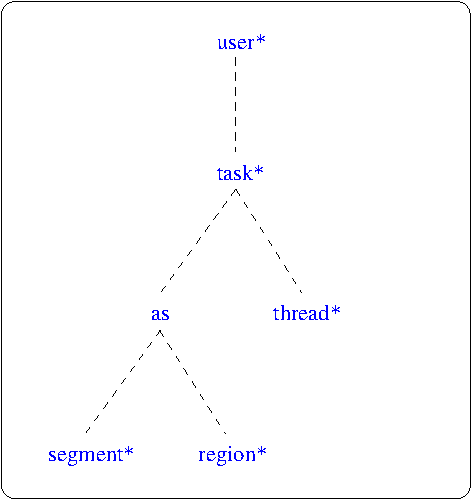
\includegraphics[scale=0.8]{figures/nomenclature_hierarchy.pdf}
    \caption{The kaneton object hierarchy.}
    \label{figure:nomenclature_hierarchy}
  \end{center}
\end{figure}

XXX est-ce que ce qui suit ne devrait pas etre mis dans coding-style ?

The kaneton core was implemented following a very strict source code
nomenclature we will now detail.

Each manager provides an interface to manipulate a kaneton object or
something else. The naming scheme used for these provided functions
is the explained below.

The function \textit{manager}\_\textbf{init}() initializes the whole
manager and the function \textit{manager}\_\textbf{clean}() cleans it.

The function \textit{manager}\_\textbf{show}() displays information
on a precise object while the function \textit{manager}\_\textbf{dump}()
displays information on every objects managed.

The function \textit{manager}\_\textbf{reserve}() reserves an object
given some properties and the function \textit{manager}\_\textbf{release}()
releases it.

The function \textit{manager}\_\textbf{clone}() clones an object. It is
important to understand that cloning an object does not just mean
generating an identical object. Indeed, cloning an object means creating
a new object with the same properties. Notice that the fact of creation
implies a new object so a new identifier.

The function \textit{manager}\_\textbf{give}() gives an object to another
entity.

The function \textit{manager}\_\textbf{flush}() cleans every objects
previously reserved depending on the implementation.

The \textit{manager} must be replaced by the manager name like \textit{as},
\textit{task}, \textit{segment} etc..

Moreover, the kaneton development environment are organized in a very
strict way to help students to find the files they are looking for. Indeed,
given a manager name \textit{manager}, the files in relation with this
manager are located in the directory listed below:

\begin{itemize}
  \item
    \textbf{kaneton/core/}\textit{manager}\textbf{/}\textit{manager}\textbf{.c}
  \item
    \textbf{kaneton/core/arch/}\textit{architecture}\textbf{/}\textit{manager}\textbf{.c}
  \item
    \textbf{kaneton/include/core/}\textit{manager}\textbf{.h}
  \item
    \textbf{kaneton/include/arch/}\textit{architecture}\textbf{/core/}\textit{manager}\textbf{.h}
\end{itemize}

%
% operating system
%

\section{Operating System}

The kaneton microkernel manages four different task classes.

A \textbf{program} is the lowest priviliged task f the system. The common
user programs are the well known UNIX{\copyright} binaries like
\textit{/bin/ls}, \textit{/bin/sh} etc..

A \textbf{service} is a microkernel server which provides a logical
service. For example, a service could be the \textit{Virtual File System}
which dispatches the calls to the filesystems to the correct servers.

A \textbf{driver} is a service which performs hardware communication.
For example, a \textit{Wireless driver} is a driver in the kaneton terms.

Finally, a \textbf{core} is a task which is a kind of super-driver in which
it has full rights on the whole machine.

A \textbf{module} is simply an additional file passed at the boot time.


%%%
%% licence       kaneton licence
%%
%% project       kaneton
%%
%% file          /home/mycure/kaneton/view/papers/kaneton/coding-style.tex
%%
%% created       matthieu bucchianeri   [mon jan 30 17:32:57 2006]
%% updated       julien quintard   [sat apr 15 22:39:02 2006]
%%

%
% coding style
%

\chapter{Coding style}

We will detail in this chapter the coding style used to develop the
kaneton microkernel reference implementation.

\newpage

%
% case
%

The kaneton project developers try to follow a coding style. This
coding style was introduced to normalize the source code, leading to a
more readable source code.

Nevertheless, you can adapt this coding style to your own but try to
follow the rules.

\section{Case}

The whole kaneton source code is written using lower case letters.

Moreover, every text including comments etc.. must be written using
lower case letters

%
% headers
%

\section{Headers}

Each file must start with a header formatted as shown below:

\begin{verbatim}
/*
 * licence       kaneton licence
 *
 * project       kaneton
 *
 * file          /home/mycure/core/kaneton/kaneton/as/as.c
 *
 * created       julien quintard   [fri feb 11 02:23:41 2005]
 * updated       matthieu bucchianeri   [mon jan 30 20:30:57 2006]
 */
\end{verbatim}

An emacs configuration file for automatically generating and updating
this header can be found in \textit{tools/emacs}.

Additionally, you need to set two environment variables to generate
a correct kaneton header:

\begin{itemize}
  \item
    \textit{EC\_LICENCE} must be set to ``kaneton licence''.
  \item
    \textit{EC\_DEVELOPER} must be set to your first name and last name.
\end{itemize}

Please, do not use nicknames in headers.

%
% naming convention
%

\section{Naming Convenions}

To keep the code as clear as possible, there are several conventions on
types, functions and variables naming.

%
% variables
%

\subsection{Variables}

Here are a few rules you are encouraged to follow:

\begin{itemize}
  \item
    \textit{sz} suffix for variables representing a size.

    \begin{verbatim}
      #define PAGESZ          4096

      int                     modsz;
    \end{verbatim}
  \item
    \textit{n} prefix for variables representing a number of objects.

    \begin{verbatim}
      int                     nclusters;
    \end{verbatim}
  \item
    etc..
\end{itemize}

Moreover, the types are used as pre-names:

\begin{verbatim}
t_vaddr                 video_vaddr;
\end{verbatim}

This example is not correct, instead prefer:

\begin{verbatim}
t_vaddr                 video;
\end{verbatim}

%
% functions
%

\subsection{Functions}

Function names must be prefixed by the file name, context name they are
implemented in.

For example, a function part of the address space manager must be prefixed
by \textit{as\_}.

These names must be chosen carefully: they must explicitely define
what the function does without being too long.

%
% types
%

\subsection{Types}

Here are the prefixes you must use when writing your own types:

\begin{itemize}
  \item
    \textit{m\_} for managers main structures.
  \item
    \textit{o\_} for kaneton objects.
  \item
    \textit{d\_} for dispatch interfaces.
  \item
    \textit{a\_} for architecture-dependent structures.
  \item
    \textit{s\_} for general purpose structures.
  \item
    \textit{t\_} for basic and general purpose typedefs.
  \item
    \textit{c\_} for kaneton capabilities.
  \item
    \textit{i\_} for kaneton identifiers.
\end{itemize}

Notice that \textit{a\_} can be combined with other prefixes, for
example \textit{ao\_} for an architecture-dependent object.

%
% includes
%

\section{Includes}

To keep the code clear and compact, developers only need to include a
minimal number of header files:

\begin{itemize}
  \item
    \textit{kaneton.h} for the microkernel declarations.
  \item
    \textit{klibc.h} for the kaneton specific C library.
\end{itemize}

These files are located in the include path, so do not use relative include
path.

\begin{verbatim}
#include <libc.h>
#include <kaneton.h>

int             main(int                argc,
                     char**             argv)
{
  [...]

  return (0);
}
\end{verbatim}

All include files must be protected against multiple inclusions. The
guard macro to use must be named using the directory name, one underscore,
the file name, one underscore and a capital ``H''.

For example, the file \textit{kaneton/include/kaneton/segment.h} will be
guarded as follow:

\begin{verbatim}
#ifndef KANETON_SEGMENT_H
#define KANETON_SEGMENT_H	1

[...]

#endif
\end{verbatim}

In addition, for architecture-dependent files, the guard macro must begin
with the architecture name; for example for the Intel architecture:
\textit{IA32\_KANETON\_SEGMENT\_H}.

%
% types
%

\section{Types}

You may use as soon as possible standard types: \textit{t\_uint8},
\textit{t\_sint32}, \textit{t\_uint64} etc..

This nomenclature is more understandable than
\textit{unsigned long long int}.

%
% return values
%

\section{Return Values}

Every function must report whether it successed or failed.

In kaneton, functions' return type must be \textit{t\_error}.

A function will return \textit{ERROR\_NONE} on success and anything
else on error, for example \textit{ERROR\_UNKNOWN} to indicate a non-specific
error.

%
% indentation
%

\section{Indentation}

There are several indentation rules in kaneton.

\begin{enumerate}
  \item
    Field names of structures and unions must be aligned with the
    structure or union name.

    \begin{verbatim}
      struct       s_set
      {
        u_set      id;
        t_setsz    size;
        t_type     type;
      };
    \end{verbatim}

    or

    \begin{verbatim}
      typedef struct
      {
        o_id       id;
        u_stats    stats;
        u_set      ass;
      }            m_as;
    \end{verbatim}
  \item
    Macros and variables must be aligned as shown below:

    \begin{verbatim}
      #define TASK_PRIOR_CORE     230
      #define TASK_HPRIOR_CORE    250
      #define TASK_LPRIOR_CORE    210

      m_task*                     task;
      u_task                      ktask = ID_UNUSED;
    \end{verbatim}

    This rule also applies for variables declarations in functions.
  \item
    Function prototypes and bodies should look like this:

    \begin{verbatim}
      t_error             stats_function(u_stats          id,
                                         char*            function,
                                         t_stats_func**   f)
      {
        t_sint64          slot = -1;
        t_sint64          i;

        [...]
      }
    \end{verbatim}

    Notice that argument names are aligned between each other,
    and variable names are aligned with function name and between
    each other.

    Try to respect this alignment between functions in a single file:
    function names may be all aligned and argument names also.
\end{enumerate}

%
% comments
%

\section{Comments}

As kaneton is intended to be a pedagogical project with clear and
understandable source code; no need to say that comments take a very
important part of this objective.

Every file must begin with a comment describing what is done in this
code via the \textit{information} section.

Moreover, every function must be preceded by a comment defining its
behavior.

For complex functions and yo prevent direct comments in the source code,
we used \textit{steps}:

\begin{itemize}
  \item
    Each critical code section in a function is preceded by a step
    number.
  \item
    The function header comment contains steps descriptions.
\end{itemize}

An example is present below:

\begin{verbatim}
/*
 * this function shows the usage of comments and steps.
 *
 * steps:
 *
 * 1) compute the index.
 * 2) make the operation.
 * 3) check the result.
 */

t_error         test_foobar(int      a,
                            int      b,
                            int*     c)
{
  int           index;

  /*
   * 1)
   */

  index = text_make_index(a, b);

  /*
   * 2)
   */

  index = index * a + b;

  /*
   * 3)
   */

  if (index < 0)
    return (ERROR_UNKNOWN);

  *c = index;

  return (ERROR_NONE);
}
\end{verbatim}

%
% sections
%

\section{Sections}

kaneton files are divided in multiple sections.

Section are delimited as shown below:

\begin{verbatim}
/*
 * ---------- includes ------------------------------------------------
 */
\end{verbatim}

Possible sections in a file are:

\begin{itemize}
  \item
    \textit{header files}: information, dependencies, defines, types,
    prototypes, macros, etc..
  \item
    \textit{source files}: information, extern, globals, includes,
    functions, etc..
  \item
    \textit{make files}: dependencies, directives, variables, rules, etc..
\end{itemize}

Moreover, every important file, for example the main file of each
kaneton manager, have to contain a section \textit{information} describing
the whole manager.

In addition, a section named \textit{assignments} is generally necessary
for manager will be filled in by the students. This section briefly describes
the work to be done by the students.

%
% macros
%

\section{Macros}

The kaneton microkernel uses few fundamental macros lited below:

\begin{itemize}
  \item
    \textit{\_\_\_bootloader} indicates that this source code belongs to
    the bootloader.
  \item
    \textit{\_\_\_kernel} indicates that this source code belongs to the
    microkernel.
  \item
    \textit{\_\_\_kaneton} indicates that this kernel is the kaneton
    microkernel.
  \item
    \textit{\_\_\_wordsz} indicates the word size: 16-bit, 32-bit,
    64-bit etc..
  \item
    \textit{\_\_\_endian} indicates the endianness.
\end{itemize}


%%%
%% licence       kaneton licence
%%
%% project       kaneton
%%
%% file          /home/buckman/kaneton/view/books/kaneton/core.tex
%%
%% created       matthieu bucchianeri   [mon jan 30 17:33:29 2006]
%% updated       matthieu bucchianeri   [wed feb  7 22:17:27 2007]
%%

%
% core
%

\chapter{Core}

In this chapter we will describe the kaneton core design and implementation.

We will precisly describe the core's managers taking care of specifying the
interface it provides.

\newpage

%
% text
%

The kaneton microkernel is composed of managers. Each manager provides
an interface to manipulate a special kaneton object or something else.

%
% id manager
%

\section{id manager}

The \textbf{id manager} provides an interface to manipulate the
kaneton identifiers.

The \textbf{id object} \textit{o\_id} is used to generate unique
- in its own name space - identifiers \textit{t\_id}.

In the current kaneton implementation, identifiers only consist in 64-bit
integers. Therefore, the id manager does not take care of identifiers
recycling. Nevertheless, the id manager interface was designed to permit
identifiers recycling.

Note that the id manager is the very first manager to be initialized. Then
the whole core will use it to generate identifiers for the other kaneton
objects.

%
% interface
%

\subsubsection{Interface}

\function{id\_show}{(o\_id* \argument{o})}
	 {
	   This function just displays the state of the id object
	   \argument{o}.
	 }

\function{id\_clone}{(o\_id* \argument{o},
                      t\_id \argument{old},
                      t\_id* \argument{new})}
	 {
	   This function duplicates an id object using the \argument{o}
	   identifier object, name space.

	   Note that cloning an identifier means reserving a new one
	   with the same properties.
	 }

\function{id\_reserve}{(o\_id* \argument{o},
                        t\_id* \argument{i})}
	  {
	    This function reserves an identifier \argument{i} using the
	    identifier object \argument{o}.
	  }

\function{id\_release}{(o\_id* \argument{o},
                        t\_id \argument{i})}
	 {
	   This function releases the identifier \argument{i}.
	 }

\function{id\_build}{(o\_id* \argument{o})}
	 {
	   This function initializes an identifier object.
	 }

\function{id\_destroy}{(o\_id* \argument{o})}
	 {
	   This function destroys an identifier object.
	 }

\function{id\_initialize}{(void)}
	 {
	   This function just initializes the id manager.
	 }

\function{id\_clean}{(void)}
	 {
	   This function just cleans the id manager.
	 }

%
% set manager
%

\section{set manager}

The \textbf{set manager} is used to manage the data structures in order
to simplify the other kernel managers. Indeed, every kernel manager
including the task manager, the thread manager, the segment manager etc.
uses the set manager to store the data rather than create and manage data
structures by their own.

More precisly, the set manager is used to store kaneton objects.
As seen earlier, kaneton objects has a first 64-bit field representing
the kaneton object's identifier. Then, the set manager uses this identifier
to retrieve an object in a set.

Notice that to avoid problems, a set must contain objects with unique
identifiers. Indeed, identifier collisions in sets are not permitted.

The set manager manages set objects. A \textbf{set object} \textit{o\_set}
is a kaneton object so is identified by a unique set identifier
\textit{i\_set}.

The set mecanism is divided in two parts: the set manager and the set
implementations.

While the set implementations are specific to each type of set: array,
linked-list, pipe, etc., the set manager code is generic and works with all
sets.

The set manager has its own nomenclature we will now detail.

The \textbf{set container} is the set which contains all the set descriptors.
Note that storing set objects in another set object is possible since
set objects are kaneton objects so have a first field kaneton identifier.

The term \textbf{set descriptor} is equivalent to the term \textit{set object}.
We use the term \textit{set object} to describe a set outside of the set
manager while the term \textit{set descriptor} is used inside the set
manager. A set descriptor contains the set meta-data. Indeed, a set descriptor
contains the number of objects managed, the set options, the size of the
objects held, the identifier of the set etc. Each set descriptor is also
composed of an implementation subpart containing the data structure holding
the objects.

A \textbf{node} is a data structure element. Indeed, each iterator
references a node to be able to locate the previous and next nodes in
the set. Note that sometimes, the node is also the object.

A \textbf{set iterator} is a pointer on a set node. Iterators were
introduced to speed up the manipulation of sets. Nevertheless, be carefull
since no insurance can be made on the coherence of iterators if set
operations are made.

To conclude on the set nomenclature, the set container is a set object
\textit{o\_set} which contains the set descriptors. Each set descriptor
\textit{o\_set} contains a data structure composed of nodes which
contain the kaneton objects provided by the set manager user.

The Figure \ref{figure:core_sets} illustrates the complex sets organization.

\begin{figure}[h]
  \begin{center}
    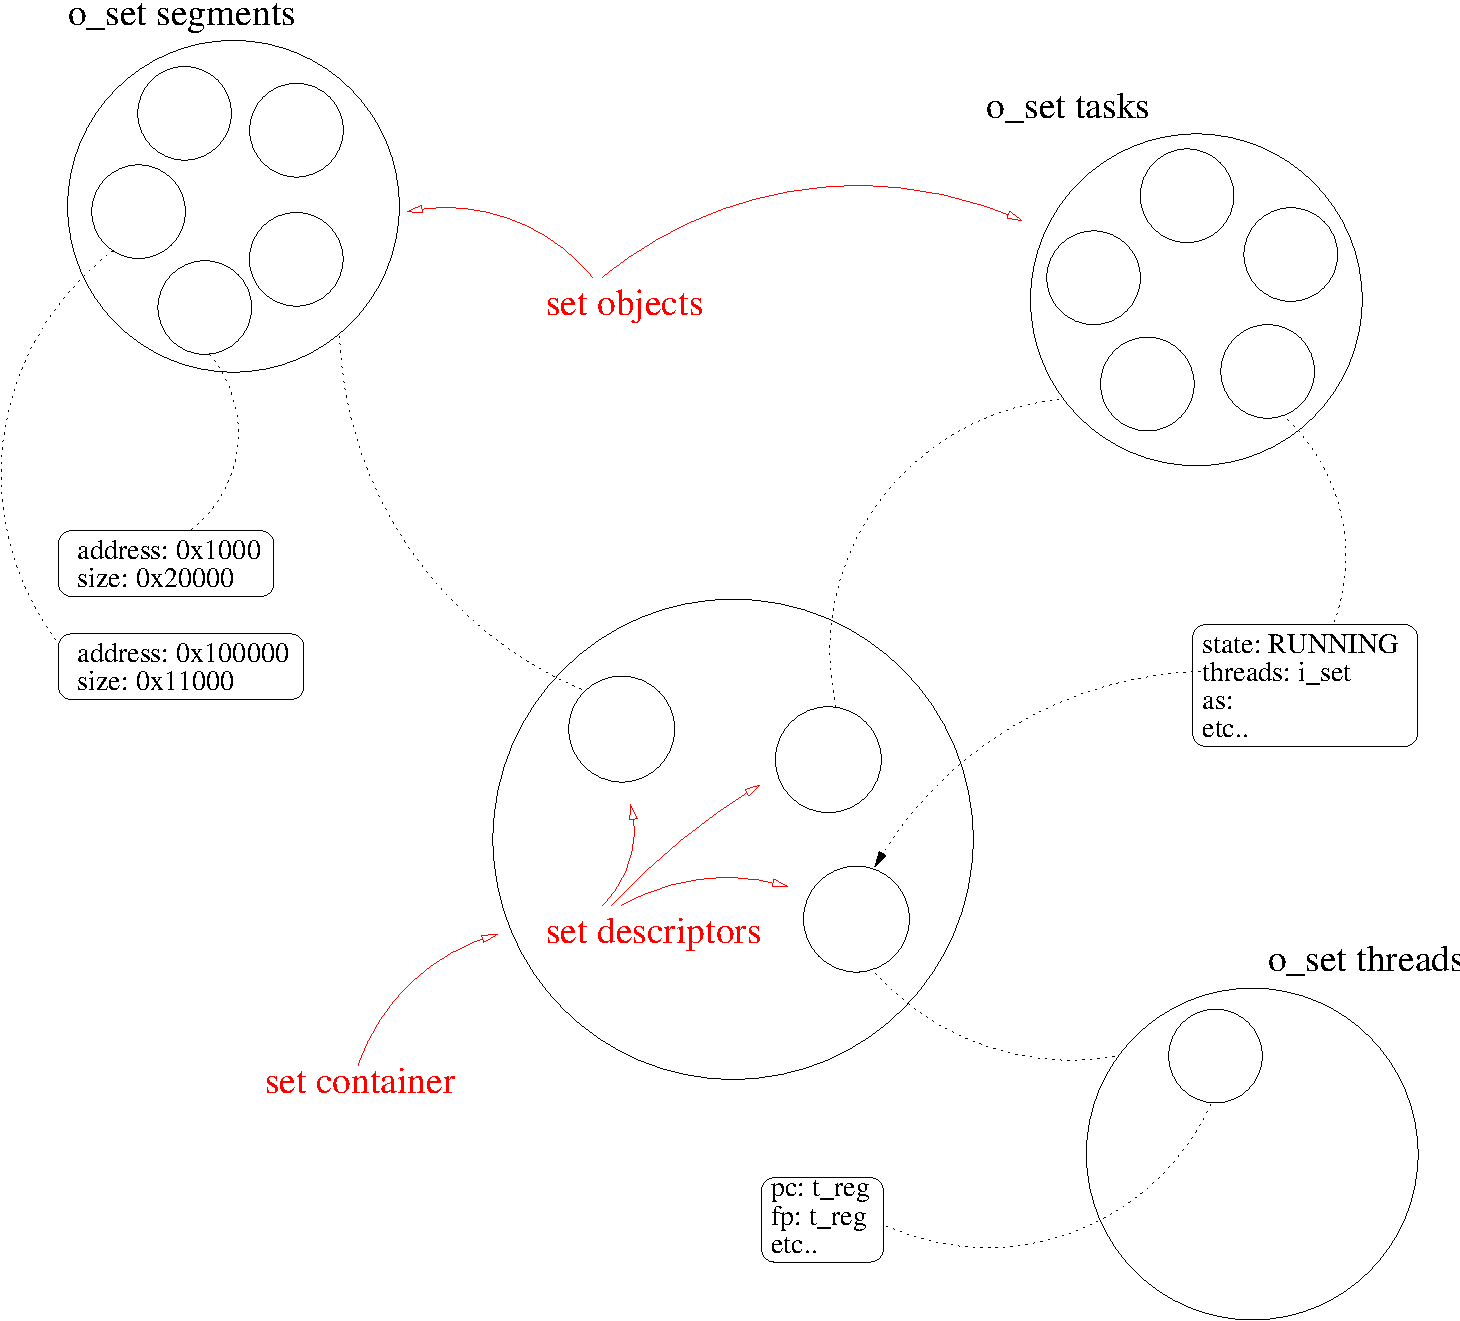
\includegraphics[scale=0.5]{figures/core_sets.pdf}
    \caption{Sets organization.}
    \label{figure:core_sets}
  \end{center}
\end{figure}

Note that the set manager is based on the \textit{malloc}() suite functions.
Indeed the set manager maintains a data structure containing the set
descriptors: the \textit{container}. Moreover some data structure
implementation require the \textit{malloc}() suite functions, the simplest
example being the array data structure which requires the \textit{realloc}()
function to be able to expand the data structure without effort.

Using this initial \textit{malloc}() function with its survival area,
the set manager is able to build sets for every kernel managers including
the segment manager, the address space manager, the region manager etc.

The set manager provides options to parameterize the set reservation.

The \textit{SET\_OPT\_CONTAINER} option is only used by the set manager
to build the very first set which then becomes the set container.

The \textit{SET\_OPT\_ALLOC} tells the set manager to always allocate
memory and to copy into this memory the content of the given object.
This option is very useful since the user never cares about allocating
memory. With this option, kaneton object stored in the set are automatically
freed when the set is released.

To tell the set manager to automatically free the objects stored without
setting the \textit{SET\_OPT\_ALLOC}, the \textit{SET\_OPT\_FREE} was
introduced. This option tells the set manager that the user will store
pre-allocated objects but the user wants them to be freed by the set
manager. This option is mutually exclusive with the
\textit{SET\_OPT\_ALLOC} option.

The \textit{SET\_OPT\_SORT} tells the set manager to always keep the set
sorted by identifiers.

The \textit{SET\_OPT\_ORGANISE} option is only used to re-organize the data
structure to keep it as simple as possible. This option may have no sens
with certain data structures.

%
% interface
%

\subsubsection{Interface}

\function{set\_type}{(i\_set \argument{id})}
	 {
	   This function just returns an error if the set corresponding
	   to \argument{id} is not of the type of the set implementation.
	 }

\function{set\_show}{(i\_set \argument{id})}
	 {
	   This function displays the entire set state of the set object
	   \argument{id}.
	 }

\function{set\_dump}{(void)}
	 {
	   This function displays all the set objects of the set manager.
	 }

\function{set\_size}{(i\_set \argument{id},
                      t\_setsz* \argument{size})}
	 {
	   This function returns in \argument{size} the number of elements
	   of the set.
	 }

\function{set\_head}{(i\_set \argument{id},
                      t\_iterator* \argument{iterator})}
	 {
	   This function returns an iterator on the first element
	   of the set \argument{id}.
	 }

\function{set\_tail}{(i\_set \argument{id},
                      t\_iterator* \argument{iterator})}
	 {
	   This function returns an iterator on the last element of
	   the set \argument{id}.
	 }

\function{set\_previous}{(i\_set \argument{id},
                          t\_iterator \argument{current},
                          t\_iterator* \argument{previous})}
	 {
	   This function returns an iterator on the previous element
	   of the set.
	 }

\function{set\_next}{(i\_set \argument{id},
                      t\_iterator \argument{current},
                      t\_iterator* \argument{next})}
	 {
	   This function returns an iterator on the next element
	   of the set.
	 }

\function{set\_insert}{(i\_set \argument{id},
                        void* \argument{data})}
	 {
	   This function inserts an object at the head of the set
	   \argument{id}.
	 }

\function{set\_append}{(i\_set \argument{id},
                        void* \argument{data})}
	 {
	   This function inserts an object at the tail of the set
	   \argument{id}.
	 }

\function{set\_before}{(i\_set \argument{id},
                        t\_iterator \argument{iterator},
                        void* \argument{data})}
	 {
	   This function inserts an object before the one specified
	   by the iterator.
	 }

\function{set\_after}{(i\_set \argument{id},
                       t\_iterator \argument{iterator},
                       void* \argument{data})}
	 {
	   This function inserts an object after the one specified
	   by the iterator.
	 }

\function{set\_add}{(i\_set \argument{id},
                     void* \argument{data})}
	 {
	   This function adds a data object in the set \argument{id}.
	 }

\function{set\_remove}{(i\_set \argument{id},
                        t\_id \argument{i})}
	 {
	   This function removes an object identified by \argument{i}
	   from the set \argument{id}.
	 }

\function{set\_delete}{(i\_set \argument{id},
                        t\_iterator \argument{iterator})}
	 {
	   This function deletes the object corresponding to the iterator.
	 }

\function{set\_flush}{(i\_set \argument{id})}
	 {
	   This function removes every object stored in the set
	   \argument{id}.
	 }

\function{set\_locate}{(i\_set \argument{id},
                        t\_id \argument{i},
                        t\_iterator* \argument{iterator})}
	 {
	   This function returns an iterator on the element corresponding
	   to the identifier \argument{i} of the set \argument{id}.
	 }

\function{set\_object}{(i\_set \argument{id},
                        t\_iterator \argument{iterator},
                        void** \argument{data})}
	 {
	   This function returns the data object corresponding to
	   the iterator.
	 }

\function{set\_push}{(i\_set \argument{id},
                      void* \argument{data})}
	 {
	   This function pushes an object into a FIFO or LIFO structure.
	 }

\function{set\_pop}{(i\_set \argument{id})}
	 {
	   This function deletes the next object of a FIFO or LIFO structure.
	 }

\function{set\_pick}{(i\_set \argument{id},
                      void** \argument{data})}
	 {
	   This function returns the next object of a FIFO or LIFO structure
	   without deleting it.
	 }

\function{set\_reserve}{(\argument{type},
                         t\_opts \argument{opts},
                         t\_size \argument{datasz},
                         i\_set* \argument{id})}
	 {
	   This function reserves a set object of type \argument{type}
	   with options \argument{opts} which will contain object of
	   \argument{datasz} size.

	   The reserved set object's identifier is returned in
	   \argument{id}.
	 }

\function{set\_release}{(i\_set \argument{id})}
	 {
	   This function releases the set \argument{id}.
	 }

\function{set\_initialize}{(void)}
	 {
	   This function initializes the set manager.
	 }

\function{set\_clean}{(void)}
	 {
	   This function cleans the set manager.
	 }

You can notice that some operations does not make sense on some data
structures. For example, \textit{set\_push}() or \textit{set\_pop}()
will never be used on arrays or lists, but only on stacks or pipes.

In these cases, the function must be implemented but will only return
an error.

Most widely, some operations have no sense with some options. Inserting
at the beginning of a sorted array must produce an error since it can
cancel the sorting property.

It is important to understand that a set implementation can specify
its own interface. Therefore, for example, the \textit{set\_reserve}()
function takes 4 arguments for the bpt implementation.

To better understand the implementations, take a look at the set
manager directory \textit{kaneton/core/set/} and its header file
\textit{kaneton/include/core/set.h}.

%
% as manager
%

\section{as manager}

The \textbf{address space manager} or \textbf{as manager} just manages
the address spaces objects.

An \textbf{address space object} or \textbf{as object} \textit{o\_as}
is an abstraction describing the addressable memory. The as objects
are identified by an address space identifier \textit{i\_as}.

An address space object is composed of a set of segments and a set of regions.

The set of segments describes the physical memory that belongs to this
address space while the set of regions describes the virtual memory
used to access the physical one.

It is important to understand that the set of segments holds segment
identifiers while the set of regions holds region objects.

%
% interface
%

\subsubsection{Interface}

\function{as\_show}{(i\_as \argument{id})}
	 {
	   This function shows a precise address space displaying
	   information on it.
	 }

\function{as\_dump}{(void)}
	 {
	   This function shows all the address space objects managed by
	   the address space manager.
	 }

\function{as\_give}{(i\_task \argument{task},
                     i\_as \argument{id})}
	 {
	   This function gives the address space \argument{id} to the
	   task object \argument{task}.
	 }

\function{as\_vaddr}{(i\_as \argument{id},
                      t\_paddr \argument{physical},
                      t\_vaddr* \argument{virtual})}
	 {
	   This function translates a physical address into its virtual
	   address.
	 }

\function{as\_paddr}{(i\_as \argument{id},
                      t\_vaddr \argument{virtual},
                      t\_paddr* \argument{physical})}
	 {
	   This function translates a virtual address into its physical
	   address.
	 }

\function{as\_read}{(i\_as \argument{asid},
		     t\_vaddr \argument{src},,
		     t\_vsize \argument{size},
		     void* \argument{dst})}
	 {
	   This function reads \argument{size} bytes at address
	   \argument{src} in the address space \argument{asid} and
	   copy them into the buffer \argument{dst}.

	   This function can read memory area spanning on multiple
	   regions and segments.

	   \note{This function is not exported by the interface
	   manager. Prefer using the \textit{as\_copy}() function.}
	 }

\function{as\_write}{(i\_as \argument{asid},
                      const void* \argument{src},
                      t\_vsize \argument{size},
                      t\_vaddr \argument{dst})}
	 {
	   This function write \argument{size} bytes of \argument{src}
	   into the address space \argument{asid} at address \argument{dst}.

	   This function can write memory area spanning on multiple
	   regions and segments.

	   \note{This function is not exported by the interface
	   manager. Prefer using the \textit{as\_copy}() function.}
	 }

\function{as\_copy}{(i\_as \argument{src\_as},
                     t\_vaddr \argument{src},
                     i\_as \argument{dst\_as},
                     t\_vaddr \argument{dst},
                     t\_vsize \argument{size})}
	 {
	   This function can copy memory areas spanning on multiple
	   regions and segments.

	   This function copies data from the address space
	   \argument{src\_as} to the address space \argument{dst\_as}.
	 }

\function{as\_clone}{(i\_task \argument{task},
                      i\_as \argument{old},
                      i\_as* \argument{new})}
	 {
	   This function clones an address space taking care of cloning
	   everything necessary: segments, regions etc.
	 }

\function{as\_reserve}{(i\_task \argument{task},
                        i\_as* \argument{id})}
	 {
	   This function reserves an address space object for the
	   task \argument{task} object.

	   The reserved address space object's identifier is returned
	   in \argument{id}.
	 }

\function{as\_release}{(i\_as \argument{id})}
	 {
	   This function just releases the address space \argument{id}.
	 }

\function{as\_get}{(i\_as \argument{id},
                    o\_as** \argument{o})}
	 {
	   This function just returns the address space object
	   corresponding to the address space identifier \argument{id}.
	 }

\function{as\_initialize}{(void)}
	 {
	   This function initializes the address space manager.
	 }

\function{as\_clean}{(void)}
	 {
	   This function cleans the address space manager.
	 }

%
% segment manager
%

\section{segment manager}

The \textbf{segment manager} manages physical memory.

Its goals is to reserve and release physical memory areas, merge or split
allocated areas and finally to read or write directly into physical memory.

The kaneton object managed by the segment manager is the segment object.

A \textbf{segment object} \textit{o\_segment} describes an area of reserved
physical memory. A segment object has some properties like the base
address, the size, the permissions etc. and is identified by a
segment identifier \textit{i\_segment}.

In the current kaneton microkernel reference implementation, the
segment object's identifier is set from the segment object's base
address. Therefore, it is so easy to retrieve segment object from
the base address. Moreover, physical address are of course unique
so the segment objects can be stored in a set object without effort.

% XXX parler des types de segments

\function{segment\_show}{(i\_segment \argument{id})}
	 {
	   This function displays information on the specified segment
	   \argument{id}.
	 }

\function{segment\_dump}{(void)}
	 {
	   This function displays all segments of the set of segments.
	 }

\function{segment\_clone}{(i\_as \argument{as},
                           i\_segment \argument{old},
                           i\_segment* \argument{new})}
	 {
	   This function clones a segment which will then belong to
	   the address space object \argument{as}.

	   Cloning a segment means reserving a new segment with the
	   exact same properties. Then the content is also copied.
	 }

\function{segment\_inject}{(i\_as \argument{as},
                            o\_segment* \argument{o},
			    i\_segment* \argument{segid})}
	 {
	   This function injects a pre-allocated segment in the set of
	   segments. The identifier of the injected segment is returned into
	   \argument{segid}.

	   \note{\textit{The given segment object must have been
	   allocated by the \textit{malloc}() function.}}
	 }

\function{segment\_give}{(i\_as \argument{as},
                          i\_segment \argument{id})}
	 {
	   This function gives a segment from one address space to another.
	 }

\function{segment\_resize}{(i\_segment \argument{old},
                            t\_psize \argument{size},
                            i\_segment* \argument{new})}
	 {
	   This function resizes the segment \argument{old} to the
	   size \argument{size}.

	   The new segment, which can be the same, is returned in
	   \argument{new}.

	   \note{This operation is not yet implemented.}
	 }

\function{segment\_split}{(i\_segment \argument{id},
                           t\_psize \argument{size},
                           i\_segment* \argument{left},
                           i\_segment* \argument{right})}
	 {
	   This function splits the segment \argument{id} into two segments.

	   The size \argument{size} specifies the size of the new left segment.

	   \note{This operation is not yet implemented.}
	 }

\function{segment\_coalesce}{(i\_segment \argument{left},
                              i\_segment \argument{right},
                              i\_segment* \argument{id})}
	 {
	   This function merges two adjacent segments into a single
	   one \argument{id}.

	   \note{This operation is not yet implemented.}
	 }

\function{segment\_read}{(i\_segment \argument{id},
                          t\_paddr \argument{offset},
                          void* \argument{buffer},
                          t\_psize \argument{size})}
	 {
	   This function reads \argument{size} bytes at offset
	   \argument{offset} from the segment \argument{id}.
	 }

\function{segment\_write}{(i\_segment \argument{id},
                           t\_paddr \argument{offset},
                           const void* \argument{buffer},
                           t\_psize \argument{size})}
	 {
	   This function write the data of \argument{buffer} into the
	   segment \argument{id}.
	 }

\function{segment\_copy}{(i\_segment \argument{dst},
                          t\_paddr \argument{offd},
                          i\_segment \argument{src},
                          t\_paddr \argument{offs},
                          t\_psize \argument{size})}
	 {
	   This function copies data from the segment \argument{src} to
	   the segment \argument{dst}.
	 }

\function{segment\_reserve}{(i\_as \argument{as},
                             t\_psize \argument{size},
                             t\_perms \argument{perms},
                             i\_segment* \argument{id})}
	 {
	   This function reserves a segment with specified properties.
	 }

\function{segment\_release}{(i\_segment \argument{id})}
	 {
	   This function releases the segment \argument{id}.
	 }

\function{segment\_catch}{(i\_as \argument{as},
                           i\_segment \argument{id})}
	 {
	   This function is used to force a segment to be given to an address
	   space.

	   \note{Catchable segments are reserved by the module service
	     for architecture specific servers. Catchable segments
	     are defined in the \argument{kaneton.conf} file.}
	 }

\function{segment\_perms}{(i\_segment \argument{id},
                           t\_perms \argument{perms})}
	 {
	   This function changes the permissions of the segment \argument{id}.
	 }

\function{segment\_type}{(i\_segment \argument{id},
                          t\_type \argument{type})}
	 {
	   This function changes the type of a segment.
	 }

\function{segment\_flush}{(i\_as \argument{as})}
	 {
	   This function removes every segment that belongs to the
	   address space \argument{as}.
	 }

\function{segment\_get}{(i\_segment \argument{id},
                         o\_segment** \argument{o})}
	 {
	   This function just returns the segment object
	   corresponding to the segment identifier \argument{id}.
	 }

\function{segment\_initialize}{(void)}
	 {
	   This function initializes the segment manager.
	 }

\function{segment\_clean}{(void)}
	 {
	   This function cleans the segment manager.
	 }

%
% region manager
%

\section{region manager}

The \textbf{region manager} manages mappings of segment called regions.

A \textbf{region object} \textit{o\_region} describes an area of virtual
memory mapping a segment part. Each region is identified by a unique region
identifier \textit{i\_region}.

As for segments, regions identifiers are set from the region base address.

\function{region\_show}{(i\_as \argument{as},
                         i\_region \argument{id})}
	 {
	   This function displays information on the specified region
	   \argument{id} of the address space object \argument{as}.
	 }

\function{region\_dump}{(i\_as \argument{as})}
	 {
	   This function displays all the regions of the address space
	   \argument{as}.
	 }

\function{region\_inject}{(i\_as \argument{as},
                           o\_region* \argument{o},
			   i\_region* \argument{regid})}
	 {
	   This function injects a pre-allocated region in the set of
	   regions of the address space \argument{as}. The identifier of
	   the injected region is returned into \argument{regid}.
	 }

\function{region\_split}{(i\_as \argument{asid},
			  i\_region \argument{regid},
			  t\_vsize \argument{size},
			  i\_region* \argument{left},
			  i\_region* \argument{right})}
	 {
	   This function split the region \argument{regid} in two regions
	   \argument{left} and \argument{right}, the left one being of size
	   \argument{size}.

	   \note{This operation is not yet implemented.}
	 }

\function{region\_resize}{(i\_as \argument{as},
                           i\_region \argument{old},
                           t\_vsize \argument{size},
                           i\_region* \argument{new})}
	 {
	   This function resizes the region \argument{old} to the
	   size \argument{size}.

	   The new region, which can be the same, is returned in
	   \argument{new}.

	   \note{This operation is not yet implemented.}
	 }

\function{region\_coalesce}{(i\_as \argument{asid},
			     i\_region \argument{left},
			     i\_region \argument{right},
			     i\_region*	\argument{regid})}
	 {
	   This function merges two neighbor regions \argument{left} and
	   \argument{right} into a single region \argument{regid}.

	   \note{This operation is not yet implemented.}
	 }

\function{region\_reserve}{(i\_as \argument{as},
                            i\_segment \argument{segment},
                            t\_paddr \argument{offset},
                            t\_opts \argument{opts},
                            t\_vaddr \argument{address},
                            t\_vsize \argument{size},
                            i\_region* \argument{id})}
	 {
	   This function reserves a region with specified properties.

	   % XXX opts
	 }

\function{region\_release}{(i\_as \argument{as},
                            i\_region \argument{id})}
	 {
	   This function releases the region \argument{id} that belongs
	   to the address space object \argument{as}.
	 }

\function{region\_flush}{(i\_as \argument{as})}
	 {
	   This function removes every region that belongs to the
	   address space \argument{as}.
	 }

\function{region\_get}{(i\_as \argument{asid},
			i\_region \argument{id},
                        o\_region** \argument{o})}
	 {
	   This function just returns the region object
	   corresponding to the region identifier \argument{id} in the
	   address space \argument{asid}.
	 }

\function{region\_initialize}{(void)}
	 {
	   This function initializes the region manager.
	 }

\function{region\_clean}{(void)}
	 {
	   This function cleans the region manager.
	 }

%
% map manager
%

\section{map manager}

It is obvious the programmer does not want to care about segments and
regions. He does not want to know what it is and why these things were
designed like that.

The programmer just wants to allocate memory. To make things easier
to the programmer, a map manager was introduced.

The \textbf{map manager} is just an abstract layer over the segment
and region manager.

Indeed its main task is to allocate memory so to reserve a segment
and a region mapping it.

%
% interface
%

\subsubsection{Interface}

\function{map\_reserve}{(i\_as \argument{as},
                         t\_opts \argument{opts},
                         t\_vsize \argument{size},
                         t\_perms \argument{perms},
                         t\_vaddr* \argument{address})}
	 {
	   This function reserves a mapping between a segment and a region.
	   The segment will have the size \argument{size} with the permissions
	   \argument{perms} while the region will map the whole segment.

	   The virtual address is returned in \argument{address}.

	   % XXX opts
	 }

\function{map\_release}{(i\_as \argument{as},
                         t\_vaddr \argument{address})}
	 {
	   This function releases a previously reserved map.
	 }

\function{map\_resize}{(i\_as \argument{asid},
			t\_vaddr \argument{old},
			t\_vsize \argument{size},
			t\_vaddr* \argument{new})}
	 {
	   This function resize the mapped area at address \argument{old}
	   to the size \argument{size}.

	   \argument{new} is the new address of the area and may not be
	   equal to the original address.

	   \note{This operation is not yet implemented.}
	 }

\function{map\_initialize}{(void)}
	 {
	   This function initializes the map manager.
	 }

\function{map\_clean}{(void)}
	 {
	   This function cleans the map manager.
	 }

%
% event manager
%

\section{event manager}

The \textbf{event manager} manages such event objects.

An \textbf{event object} \textit{o\_event} is an abstraction over the
well-known hardware and software interrupts. Each event object is
identified by a unique event identifier \textit{i\_event}.

The events are used to describe a behaviour and to associate an action
to them.

Then, every time an hardware or software interrupt is triggered, the
architecture dependent code will pass on the information to the core
which will perform the associate action.

The common actions are either to run a specific event handler or to
send an event message to a specific kaneton task.

%
% interface
%

\function{event\_show}{(i\_event \argument{id})}
	 {
	   This function displays information on an event object.
	 }

\function{event\_dump}{(void)}
	 {
	   This function displays information on all the event objects.
	 }

\function{event\_reserve}{(i\_event \argument{id},
                           t\_type \argument{type},
                           u\_event\_handler \argument{handler},
			   t\_vaddr \argument{data})}
	 {
	   This function installs an event handler. The \argument{data}
	   value will be passed as an argument of the handler.

	   The handler \argument{handler} is a function pointer when
	   \argument{type} is EVENT\_FUNCTION or a task identifier when
	   \argument{type} is EVENT\_MESSAGE.
	 }

\function{event\_release}{(i\_event \argument{id})}
	 {
	   This function releases an event object.
	 }

\function{event\_get}{(i\_event \argument{id},
                       o\_event** \argument{o})}
	 {
	   This function returns in \argument{o} the event object
	   corresponding to \argument{id}.
	 }

\function{event\_initialize}{(void)}
	 {
	   This function initializes the event manager.
	 }

\function{event\_clean}{(void)}
	 {
	   This function cleans the event manager.
	 }

%
% timer manager
%

\section{timer manager}

The \textbf{timer manager} manages timer objects.

A \textbf{timer object} \textit{o\_timer} is a timed event that measures
relative time. Each timer object is identified by a unique timer identifier
\textit{i\_timer}.

%
% interface
%

\function{timer\_show}{(i\_timer \argument{id})}
	 {
	   This function displays information on a timer object.
	 }

\function{timer\_dump}{(void)}
	 {
	   This function displays information on all the timers.
	 }

\function{timer\_reserve}{(t\_type \argument{type},
			   u\_timer\_handler \argument{handler},
			   t\_vaddr \argument{data},
                           t\_uint32 \argument{delay},
                           t\_uint32 \argument{repeat},
                           i\_timer* \argument{id})}
	 {
	   This function reserves a timer which will expire in
	   \argument{delay} microseconds.

	   The \argument{repeat} argument specifies if the timer
	   must be re-inserted once expired. % XXX macro

	   The \argument{data} value will be passed as an argument
	   of the handler.

	   The handler \argument{handler} is a function pointer when
	   \argument{type} is EVENT\_FUNCTION or a task identifier when
	   \argument{type} is EVENT\_MESSAGE.
	 }

\function{timer\_release}{(i\_timer \argument{id})}
	 {
	   This function releases a timer object.
	 }

\function{timer\_delay}{(i\_timer \argument{id},
                         t\_uint32 \argument{delay})}
	 {
	   This function updates the delay of the timer \argument{id}.
	 }

\function{timer\_repeat}{(i\_timer \argument{id},
                          t\_uint32 \argument{repeat})}
	 {
	   This function updates the repeat property of the timer
	   \argument{id}. % XXX macro
	 }

\function{timer\_modify}{(i\_timer \argument{id},
			  t\_uint32 \argument{delay},
			  t\_uint32 \argument{repeat})}
	 {
	   This function updates both the timer delay and repeat property
	   of the timer \argument{id}. % XXX macro
	 }

\function{timer\_get}{(i\_timer \argument{id},
                       o\_timer** \argument{o})}
	 {
	   This function returns in \argument{o} the timer object
	   corresponding to \argument{id}.
	 }

\function{timer\_initialize}{(void)}
	 {
	   This function initializes the timer manager.
	 }

\function{timer\_clean}{(void)}
	 {
	   This function cleans the timer manager.
	 }

%
% task manager
%

\section{task manager}

The \textbf{task manager} provides a complete interface for the task
objects manipulation.

A \textbf{task object} \textit{o\_task} describes a complete execution
entity. Nevertheless, a task object is never scheduled since a task
is not an active entity.

A task is composed of an address space \textit{o\_as} and threads
\textit{o\_thread}.

Be careful, a task in the kaneton terms is different from a \textit{process}
in the UNIX{\copyright} terms. Indeed, a \textit{process} has only one
thread while kaneton tasks can have multiple ones. Nevertheless, the
term \textit{process} is sometimes used to describe a kaneton task.

Each task is identified by a unique task identifier \textit{i\_task}.

The task manager uses an internal nomenclature we will now detail.

The \textbf{class} \textit{t\_class} describes the task's rights on the
system. The different classes are \textit{TASK\_CLASS\_CORE},
\textit{TASK\_CLASS\_DRIVER}, \textit{TASK\_CLASS\_SERVICE} and
\textit{TASK\_CLASS\_PROGRAM}.

So a kaneton \textit{service} is in fact a task with a class
\textit{TASK\_CLASS\_SERVICE} and so on for the \textit{core},
\textit{drivers} and \textit{programs}.

These classes permit to give certain tasks, for example, the permission
to interact with hardware devices.

Moreover, this classification permit to build a tasks hierarchy.
Therefore, a task will be authorized to call another task only if
greater or equal privileged.

\note{This calls hierarchy must be validated.}

The \textbf{behaviour} \textit{t\_behav} describes a priority
interval, each task being able to evolve in it by itself. The different
behaviors are \textit{TASK\_BEHAV\_CORE}, \textit{TASK\_BEHAV\_REALTIME},
\textit{TASK\_BEHAV\_INTERACTIVE}, \textit{TASK\_BEHAV\_TIMESHARING}
and \textit{TASK\_BEHAV\_BACKGROUND}.

The \textbf{priority} \textit{t\_prior} specify the current task
priority. Then, a task can updates its priority while this new priority
still is in the behaviour priority interval.

%
% interface
%

\subsubsection{Interface}

\function{task\_show}{(i\_task \argument{id})}
	 {
	   This function displays information on the task \argument{id}.
	 }

\function{task\_dump}{(void)}
	 {
	   This function displays information on every task.
	 }

\function{task\_current}{(i\_task* \argument{id})}
	 {
	   This function identifies which task is currently running
	   on the calling cpu.
	 }

\function{task\_clone}{(i\_task \argument{old},
                        i\_task* \argument{new})}
	 {
	   This function clones a task.

	   This function must take care of cloning everything necessary
	   including the address space and the threads.
	 }

\function{task\_reserve}{(t\_class \argument{class},
                          t\_behav \argument{behav},
                          t\_prior \argument{prior},
                          i\_task* \argument{id})}
	 {
	   This function reserves a task object with the given
	   properties: \argument{class}, \argument{behav} and
	   \argument{prior}.

	   Note that once reserved, the task is marked as stopped.

	   % XXX macros
	 }

\function{task\_release}{(i\_task \argument{id})}
	 {
	   This function releases the task object \argument{id}.
	 }

\function{task\_priority}{(i\_task \argument{id},
                           t\_prior \argument{prior})}
	 {
	   This function updates the task's priority to \argument{prior}.
	 }

\function{task\_state}{(i\_task \argument{id},
			t\_state \argument{state})}
	 {
	   This function update the state of the task \argument{id}.

	   % XXX macros
	 }

\function{task\_wait}{(i\_task \argument{id},
                       t\_opts \argument{opts},
                       t\_wait* \argument{wait})}
	 {
	   This function waits for state change in one or more tasks
	   depending on the options \argument{opts}.

	   The flags of \argument{opts} specify the state to wait for:
	   \textit{WAIT\_DEATH}, \textit{WAIT\_START},
	   \textit{WAIT\_STOP} and \textit{WAIT\_ALL}.

	   Moreover, other flags are used to precise the tasks to wait for:
	   \textit{WAIT\_ID} for a precise task \argument{id} or
	   \textit{WAIT\_CHILDREN} for any children.

	   Finally, another flag \textit{WAIT\_NOHANG} can be used
	   to make the function non-blocking if no task's state has changed.

	   \note{All these features are not implemented yet.}

	   \note{We could probably extend the waiting states to more
	     exotic ones like WAIT\_IO etc.}
	 }

\function{task\_get}{(i\_task \argument{id},
                      o\_task** \argument{o})}
	 {
	   This function returns in \argument{o} the task object corresponding
	   to \argument{id}.
	 }

\function{task\_initialize}{(void)}
	 {
	   This function initializes the task manager.
	 }

\function{task\_clean}{(void)}
	 {
	   This function cleans the task manager.
	 }

%
% thread manager
%

\section{thread manager}

The \textbf{thread manager} manages the real active execution context
called threads.

A \textbf{thread object} is an active entity which describes the
current state of an execution context including the \textit{program counter},
the \textit{stack pointer} etc.

Indeed, a thread is composed of a current \textit{program counter} which
keeps the next instruction address to execute and the \textit{stack pointer}
which keeps the stack address. With these two characteristics, a thread
can be described.

Needless to say, some additional architecture-dependent properties are
required to fully describe a thread context.

Like the tasks, each thread has its own priority meaning that each thread
can parameterize its scheduling priority.

The threads' priorities must be contained in the interval $[10, 250[$, the
macro \textit{THREAD\_PRIOR} representing the default priority.

%
% interface
%

\subsubsection{Interface}

\function{thread\_show}{(i\_thread \argument{id})}
	 {
	   This function displays information on the thread \argument{id}.
	 }

\function{thread\_dump}{(void)}
	 {
	   This function displays information on all the threads.
	 }

\function{thread\_give}{(i\_task \argument{task},
                         i\_thread \argument{id})}
	 {
	   This function gives the thread object \argument{id} to the
	   task \argument{task}.
	 }

\function{thread\_clone}{(i\_task \argument{task},
                          i\_thread \argument{old},
                          i\_thread* \argument{new})}
	 {
	   This function clones the task \argument{old} into a new one
	   \argument{new}.

	   This new thread, having the exact same properties as \argument{old},
	   will be held by the task \argument{task}.
	 }

\function{thread\_reserve}{(i\_task \argument{task},
                            t\_prior \argument{prior},
                            i\_thread* \argument{id})}
	 {
	   This function reserves a thread for the task \argument{task}
	   given the default thread priority \argument{prior}.

	   Note that once reserved, the thread is marked as stopped.
	 }

\function{thread\_release}{(i\_thread \argument{id})}
	 {
	   This function releases the thread object \argument{id}.
	 }

\function{thread\_priority}{(i\_thread \argument{id},
                             t\_prior \argument{prior})}
	 {
	   This function updates the current thread priority
	   to \argument{prior}.
	 }

\function{thread\_state}{(i\_thread \argument{id},
			  t\_state \argument{state})}
	 {
	   This function change the state of the thread \argument{id}.

	   % XXX macros
	 }

\function{thread\_stack}{(i\_thread \argument{id},
                          t\_vsize \argument{size})}
	 {
	   This function allocates a stack of \argument{size} bytes
	   for the thread \argument{id}.

	   % XXX prototype
	 }

\function{thread\_args}{(i\_thread \argument{id},
                         const void* \argument{args},
                         t\_size \argument{size})}
	 {
	   This function installs the arguments of the thread \argument{id}
	   on its stack.

	   In other words, this function copies \argument{size} bytes
	   from \argument{args} on the thread's stack.

	   Note that this function was designed to fit the general case.
	   Indeed, the special case of the \textit{main}() function
	   with its arguments \textit{argc} and \textit{argv} is not
	   directly handled by this function.

	   A C library function must be used to pack command line
	   argument strings into a unique arguments array. Then the
	   \textbf{thread\_args}() function can be used to install
	   this array onto the stack.
	 }

\function{thread\_wait}{(i\_thread \argument{id},
                         t\_opts \argument{opts},
                         t\_wait* \argument{wait})}
	 {
	   This function acts like the function \textbf{task\_wait}().

	   This function waits for the thread's state to change depending on
	   the options \argument{opts}.

	   \note{This operation is not yet implemented.}
	 }

\function{thread\_flush}{(i\_task \argument{task})}
	 {
	   This function removes every thread that belongs to the
	   task object \argument{task}.
	 }

\function{thread\_load}{(i\_thread \argument{id},
                         t\_thread\_context \argument{context})}
	 {
	   This function loads a new execution context in the thread
	   object \argument{id}.

	   A thread execution context \textit{t\_thread\_context}
	   only contains the \textit{program counter} and the
	   \textit{stack pointer}.
	 }

\function{thread\_store}{(i\_thread \argument{id},
                          t\_thread\_context* \argument{context})}
	 {
	   This function stores in \argument{context} the current
	   thread execution context of the thread object \argument{id}.
	 }

\function{thread\_get}{(i\_thread \argument{id},
                        o\_thread** \argument{o})}
	 {
	   This function returns in \argument{o} the thread object
	   corresponding to \argument{id}.
	 }

\function{thread\_initialize}{(void)}
	 {
	   This function initializes the thread manager.
	 }

\function{thread\_clean}{(void)}
	 {
	   This function cleans the thread manager.
	 }

%
% scheduler
%

\section{scheduler}

The \textbf{scheduler}'s role is to schedule the threads' execution
based on some properties like the tasks' behaviors, the tasks' priorities
and the threads' priorities.

Be careful, the scheduler schedules the threads which are the active
execution entities and not the tasks.

Current implementation of the scheduler uses a multilevel feedback
queues algorithm. The scheduler, in conjunction with the \textbf{cpu
manager}, supports multiple processors.

%
% interface
%

\subsubsection{Interface}

\function{scheduler\_quantum}{(t\_quantum \argument{quantum})}
	 {
	   This function sets the scheduler quantum to \argument{quantum}.
	 }

\function{scheduler\_yield}{(i\_cpu \argument{cpuid})}
	 {
	   This function permits the current task to relinquish
	   the processor \argument{cpuid} voluntarily.
	 }

\function{scheduler\_add}{(i\_thread \argument{thread})}
	 {
	   This function adds a runnable thread to the scheduler.
	 }

\function{scheduler\_remove}{(i\_thread \argument{thread})}
	 {
	   This function remove a thread from the scheduler.
	 }

\function{scheduler\_update}{(i\_thread \argument{thread})}
	 {
	   This function asks the scheduler to update the thread
	   \argument{thread} in its internal data structures since
	   for example the thread's priority just changed.
	 }

\function{scheduler\_current}{(i\_thread* \argument{thread})}
	 {
	   This function returns in \argument{thread} the identifier
	   of the thread currently executed on the current processor.
	 }

\function{scheduler\_switch}{(void)}
	 {
	   This function just elects and schedules a new runnable thread.
	 }

\function{scheduler\_initialize}{(void)}
	 {
	   This function initializes the scheduler.
	 }

\function{scheduler\_clean}{(void)}
	 {
	   This function cleans the scheduler.
	 }

%
% scheduler
%

\section{cpu manager}

The \textbf{cpu manager} provides all mecanisms to support
symmetrical multiprocessor platforms.

The interface of this manager provides functions to assign a processor
to a newly created task, to migrate a task from one processor to
another and to perform load-balancing.

A \textbf{cpu object} contains information dealing about a
microprocessor's load weight and efficiency. These statistics are
updated by the scheduler, which reports the current activity of each
processors (like the effective timeslice of a thread on a given
microprocessor.

%
% interface
%

\subsubsection{Interface}

\function{cpu\_show}{(i\_cpu \argument{id})}
	 {
	   This function displays information on the processor \argument{id}.
	 }

\function{cpu\_dump}{(void)}
	 {
	   This function displays information on all the active
	   microprocessors.
	 }

\function{cpu\_current}{(i\_cpu* \argument{id})}
	 {
	   This function sets \argument{id} to the identifier of the
	   microprocessor on which the kernel is currently running.
	 }

\function{cpu\_select}{(i\_cpu* \argument{id})}
	 {
	   This function is called when a new task is created. It gives
	   the identifier of the microprocessor with the lowest load.

	   \note{This operation is not yet implemented.}
	 }

\function{cpu\_stats}{(i\_cpu \argument{id},
                       t\_timeslice \argument{time})}
	 {
	   This function updates statistics for the processor \argument{id}.

	   \note{This function will be extended to provide more
	   precise statistics.}
	 }

\function{cpu\_balance}{(void)}
	 {
	   This function -- called periodically -- performs a
	   load-balancing on all processors.

	   \note{This operation is not yet implemented.}
	 }

\function{cpu\_migrate}{(i\_task \argument{tskid},
                         i\_cpu \argument{destination})}
	 {
	   This function migrates the task \argument{tskid} to the
	   processor \argument{destination}.
	 }

\function{cpu\_get}{(i\_cpu \argument{id},
                     o\_cpu** \argument{o})}
	 {
	   This function get the object corresponding to the processor
	   \argument{id}.
	 }

\function{cpu\_initialize}{(void)}
	 {
	   This function initializes the cpu manager.
	 }

\function{cpu\_clean}{(void)}
	 {
	   This function cleans the cpu manager.
	 }

\note{The cpu manager is not yet finished. For the moment, it only
supports a single microprocessor.}

%
% message manager
%

\section{message manager}

The \textbf{message manager} provides a complete interface to send and
receive messages in many different ways.

The kaneton message interface directly comes from standards in parallel
and distributed programming.

The message manager provides blocking and non-blocking functions,
synchronous and asynchronous messages etc.

A synchronous function is a function which does not permit the calling
task to execute instructions until the message is fully copied to the
destination buffer.

In a performance perpective, in Kaneton, kernel bufferization is avoided
as much as possible.

A blocking function is a function which does not return until the
action is totally performed. As a non-blocking function does not certify
that the action has been performed when the function returns, that is to
say we don't know if the given buffer has been entirely read/written. With
non-blocking functions, sending/receiving buffers are not securely accessible
until we are not assured that the message is copied somewhere. Functions
\textit{message\_wait}() and \textit{message\_status}() are provided for
this.

The messaging primitives are accessible from userspace through syscalls,
functions parameters are passed through CPU registers. Messages bound for
the kernel are directly redirected to the interface manager.

Each messages has a type which is associated with a message size. For each
tasks, used types must be registered.

\note{The system calls corresponding to these functions do not take
the first argument, which is in all cases an \argument{i\_task}}

%
% interface
%

\subsubsection{Interface}

\function{message\_register}{(i\_task \argument{task},
			      t\_type \argument{type},
			      t\_vsize \argument{size})}
	 {
	   This function registers for the task \argument{task} the type
	   of message \argument{type} for which the maximum size is
	   \argument{size} bytes long.
	 }

\function{message\_flush}{(i\_task \argument{task})}
	 {
	   This function flushes all the messages awaiting for delivery
	   in the task \argument{task}.
	 }

\function{message\_send}{(i\_task \argument{task},
			  i\_node \argument{destination},
			  t\_type \argument{type},
			  t\_vaddr \argument{data},
			  t\_vsize \argument{size})}
	 {
	   This blocking function performs an asynchronous send of the
	   message of registered type \argument{type} located at
	   \argument{data} of size \argument{size} to the node
	   \argument{destination} in the distributed system.
	 }

\function{message\_transmit}{(i\_task \argument{task},
			      i\_node \argument{destination},
			      t\_type \argument{type},
			      t\_vaddr \argument{data},
			      t\_vsize \argument{size})}
	 {
	   This blocking function performs a synchronous send of the
	   message of registered type \argument{type} located at
	   \argument{data} of size \argument{size} to the node
	   \argument{destination} in the distributed system.
	 }

\function{message\_throw}{(i\_task \argument{task},
			   i\_node \argument{destination},
			   t\_type \argument{type},
			   t\_vaddr \argument{data},
			   t\_vsize \argument{size},
			   t\_message\_request* \argument{request})}
	 {
	   This blocking function performs an asynchronous send of the
	   message of registered type \argument{type} located at
	   \argument{data} of size \argument{size} to the node
	   \argument{destination} in the distributed system.

	   The \argument{request} argument will be needed after the call
	   to control the completeness of the operation.

	   \note{On uniprocessor systems, this function is simply an
	     alias to \argument{message\_send()}}

	   \note{This operation is not yet implemented.}
	 }

\function{message\_receive}{(i\_task \argument{task},
			     t\_type \argument{type},
			     t\_vaddr \argument{data},
			     i\_node* \argument{sender})}
	 {
	   This blocking function waits (stop calling thread execution)
	   until a message of register type \argument{type} is received.
	   The message content is copied at address \argument{data} and
	   the sender is returned in \argument{sender}.
	 }

\function{message\_poll}{(i\_task \argument{task},
			  t\_type \argument{type},
			  t\_vaddr \argument{data},
			  i\_node* \argument{sender})}
	 {
	   This blocking function look for a message of register type
	   \argument{type} being received, and otherwise returns an error.
	   The message content is copied at address \argument{data} and
	   the sender is returned in \argument{sender}.
	 }

\function{message\_grab}{(i\_task \argument{task},
			  t\_type \argument{type},
			  t\_vaddr \argument{data},
			  i\_node* \argument{sender},
			  t\_message\_request* \argument{request})}
	 {
	   This non-blocking function receives a message of register
	   type \argument{type}.
	   The message content is copied at address \argument{data} and
	   the sender is returned in \argument{sender}.

	   The argument \argument{request} is later used to check the
	   status of the operation.

	   \note{On uniprocessor systems, this function is simply an
	     alias to \argument{message\_receive()}}

	   \note{This operation is not yet implemented.}
	 }

\function{message\_wait}{(i\_task \argument{task},
			  t\_message\_request \argument{request})}
	 {
	   This function blocks the calling task until the message request
	   described by \argument{request} is fully completed.

	   \note{This operation is not yet implemented.}
	 }


\function{message\_state}{(i\_task \argument{task},
			   t\_message\_request \argument{request})}
	 {
	   This function returns whether the message request described
	   by \argument{request} is fully completed or not.

	   \note{This operation is not yet implemented.}
	 }

\function{message\_initialize}{(void)}
	 {
	   This function initializes the message manager.
	 }

\function{message\_clean}{(void)}
	 {
	   This function cleans the message manager.
	 }

\begin{comment}


\end{comment}

%
% io manager
%

\section{io manager}

The \textbf{io manager} provides an interface to interact with
hardware through the microprocessor I/O ports or through memory mapped
I/O.

We use the term ``I/O port'', even if it refers to memory-mapped I/O
depending on the architecture.

The control of I/O ports access is implemented \textit{via} a couple
of functions that allow or deny one precise task from reading or
writing to a port. There is no way to deny a given operation (eg:
reading or writing).

The read and write operations are performed by the io manager
architecture dependent part.

%
% interface
%

\subsubsection{Interface}

\function{io\_grant}{(i\_port \argument{id},
                      i\_task \argument{task},
                      t\_uint8 \argument{width})}
	 {
	   This function grant \argument{task} for accessing
	   \argument{width} bytes of \argument{id} port both for
	   reading and writing.
	 }

\function{io\_deny}{(i\_port \argument{id},
                     i\_task \argument{task},
                     t\_uint8 \argument{width})}
	 {
	   This function deny \argument{task} for accessing
	   \argument{width} bytes of \argument{id} port both for
	   reading and writing.
	 }

\function{io\_read\_8}{(i\_task \argument{task},
                        i\_port \argument{id},
                        t\_uint8* \argument{data})}
	 {
	   This function reads a byte from \argument{id} port for
	   \argument{task}.
         }

\function{io\_read\_16}{(i\_task \argument{task},
                         i\_port \argument{id},
                         t\_uint16* \argument{data})}
	 {
	   This function reads a 16 bits word from \argument{id} port for
	   \argument{task}.
         }

\function{io\_read\_32}{(i\_task \argument{task},
                         i\_port \argument{id},
                         t\_uint32* \argument{data})}
	 {
	   This function reads a 32 bits word from \argument{id} port for
	   \argument{task}.
         }

\function{io\_read\_64}{(i\_task \argument{task},
                         i\_port \argument{id},
                         t\_uint64* \argument{data})}
	 {
	   This function reads a 64 bits word from \argument{id} port for
	   \argument{task}.
         }

\function{io\_write\_8}{(i\_task \argument{task},
                         i\_port \argument{id},
                         t\_uint8 \argument{data})}
	 {
	   This function write a byte to \argument{id} port for
	   \argument{task}.
         }

\function{io\_write\_16}{(i\_task \argument{task},
                          i\_port \argument{id},
                          t\_uint16 \argument{data})}
	 {
	   This function write a 16 bits word to \argument{id} port for
	   \argument{task}.
         }

\function{io\_write\_32}{(i\_task \argument{task},
                          i\_port \argument{id},
                          t\_uint32 \argument{data})}
	 {
	   This function write a 32 bits word to \argument{id} port for
	   \argument{task}.
         }

\function{io\_write\_64}{(i\_task \argument{task},
                          i\_port \argument{id},
                          t\_uint64 \argument{data})}
	 {
	   This function write a 64 bits word to \argument{id} port for
	   \argument{task}.
         }

\function{io\_initialize}{(void)}
	 {
	   This function initializes the io manager.
	 }

\function{io\_clean}{(void)}
	 {
	   This function cleans the io manager.
	 }

\note{All read/write functions may not be implemented depending of
the architecture.}


%%
% ---------- header -----------------------------------------------------------
%
% project       kaneton
%
% license       kaneton
%
% file          /home/mycure/kaneton/view/book/development/tools.tex
%
% created       julien quintard   [sun may 20 14:48:11 2007]
% updated       julien quintard   [sun may 20 15:22:11 2007]
%

%
% ---------- tools ------------------------------------------------------------
%

\chapter{Tools}

This chapter describes every tool kaneton contributors use on a daily-basis.

\newpage

%
% ---------- text -------------------------------------------------------------
%

%
% internal
%

\section{Internal}

%
% ---------- header -----------------------------------------------------------
%
% project       kaneton
%
% license       kaneton
%
% file          /home/mycure/kaneton/view/book/development/environment.tex
%
% created       julien quintard   [sun may 20 14:49:26 2007]
% updated       julien quintard   [thu jun 12 11:06:22 2008]
%

%
% ---------- environment ------------------------------------------------------
%

\subsection{Environment}
\label{section:environment}

Over the years, the kaneton microkernel evolved, starting with a very simple
introduction to low-level programming and finally to a complete microkernel
development.

kaneton people wanted to lead students to a complete microkernel development
to finally introduce distributed computing. This would not have been possible
if students had to build an entire development environment because developing
such an environment is a whole project by itself.

As a result, kaneton people decided to provide students a complete development
environment. The kaneton development environment is composed of make files,
python scripts and configuration files. This development environment can be
considered as one of the major kaneton tools since contributors use it
everytime.

The kaneton development environment aims at providing an easy and portable
way for managing the kaneton microkernel project from a development point
of view. Therefore, the kaneton environment provides everything necessary
for compiling, assembling, \etc{} These tasks highly rely on the underlying
running operating system as well as on the kaneton microkernel's target
microprocessor. Moreover, the user could need to redefine some behaviours
depending on its personal operating system configuration to use a specific
C compiler for instance.

The kaneton development environment provides a layered organisation of
profiles, each profile defining variables and functions used by the final
environment engine. The goal of the layered model is to allow layers to
override the definitions of lower-level layers.

%
% profiles
%

\subsubsection{Profiles}

The development environment is composed of profiles including a \name{host}
profile which describes the behaviour of the underlying operating system, a
\name{kaneton} profile which parameters the kaneton microkernel and a
\name{user} profile which permits the user to redefine lower-level layers'
declarations.

These profiles eventually hold sub-profiles which define variables and
functions. These actual profiles are accessed according to user-defined
shell variables.

% host

\subsubsubsection{Host}

The \name{host} profile essentially describes how to perform basic tasks:
compile, assemble, change the current directory, display a message \etc{} These
tasks rely on the operating system currently running as well as on the target
processor which kaneton will be built for. For these reasons, there are
several host sub-profiles.

Let us suppose a developer is running a \name{Linux} operating system and
that kaneton will be built for running on a \name{PowerPC} microprocessor. In
such a case, the C compiler program will be different depending on the
microprocessor \name{Linux} is running on. Indeed, if Linux is running on
a \name{PowerPC} microprocessor, then using the default compiler should
produce \name{PowerPC} object files. This is well-known to be the common
compiling way. On the other hand, if \name{Linux} is running on a
different microprocessor, then a cross-compiler must be used to produce
binary objects targeting a specific different microprocessor architecture,
the \name{PowerPC} architecture in our example.

To avoid this issue, a \name{host} sub-profile name is composed of two parts
separated by a slash. The first part is the name of the operating system and
the latter is a pair source/target processors separated by a period. For
example, \name{linux/ia32.ppc} names a \name{host} profile representing a
\name{Linux} operating system on a \name{Intel 32-bit} microprocessor
which aims at building a kaneton microkernel for a \name{PowerPC}
target architecture. Needless to say that \name{linux/ia32.ia32} represents
a non cross-compiling environment.

To avoid configuration duplications, it is common to see the configuration
file of a host sub-profile to include files of the parent directory as
shown below:

\begin{verbatim}
  linux/
    linux.desc
    linux.conf
    linux.mk
    linux.py
    ia32.ia32/
      educational -> .
      optimised -> .
      smp -> .
      ia32.desc
      ia32.conf
      ia32.mk
      ia32.py
    ia32.mips64/
      mips64.desc
      mips64.conf
      mips64.mk
      mips64.py
\end{verbatim}

Note that the files \location{linux.*} are not directly included by the
development environment engine since \name{linux} is not a valid host
profile name.

Two host profiles are illustrated here. The first one is named
\name{linux/ia32.ia32} while the second's name is \name{linux/ia32.mips64}.

For example, the \name{linux/ia32.mips64} \name{host} profile represents a
\name{Linux} operating system running on a \name{Intel 32-bit}
microprocessor while kaneton is built for a \name{MIPS 64-bit} target
architecture. This profile is likely to include the \location{linux.*} files
of the parent directory since there are not much difference between all the
\name{linux/*.*} \name{host} profiles. However, such a profile will
certainly redefine the binary paths of the C compiler, linker \etc{} in order
to produce \name{MIPS 64-bit} binary objects.

To conclude, the \name{host} sub-profile is accessed by the following
construct:

\begin{verbatim}
  profile/host/${KANETON_HOST}/${KANETON_ARCHITECTURE}
\end{verbatim}

With, for instance, the following values:

\begin{verbatim}
  KANETON_HOST = linux/ia32
  KANETON_ARCHTECTURE = ia32/educational
\end{verbatim}

Note that the possibility to include files in the configuration syntax allows
very similar profiles to share a huge amount of definitions.

% kaneton

\subsubsubsection{kaneton}

The \name{kaneton} profile is composed of four sub-profiles: \name{core},
\name{platform}, \name{architecture} and \name{libc}.

The \name{core} sub-profile contains variables for parameterizing the
kaneton core. The \name{platform} and \name{architecture} sub-profiles
focus on the configuration of the platform- and architecture-dependent code
of the kaneton microkernel, respectively. The \name{libc} sub-profile
contains parameters for the \name{C Library} used in the kernel.

The user-defined shell variables \code{\$\{KANETON\_PLATFORM\}} and
\code{\$\{KANETON\_ARCHITECTURE\}} are used to address the \name{platform}
and \name{architecture} sub-profiles, respectively.

% user

\subsubsubsection{User}

Let us suppose that a developer would like the kaneton microkernel to
use a specific memory management entirely based on a \name{Slab Allocator}
and with all microprocessor optimisations enabled. These user-specific
configurations are actually allowed by the \name{user} profile.

The user-defined shell variable \code{\$\{KANETON\_USER\}} defines the name
of the \name{user} profile. This profile contains user-specific
configurations allowing a contributor to overwrite lower-level layer defintions
in order to specialise a behaviour.

The kaneton project also provides a tool allowing users to configure
their development environment. This tool is named \name{configure} and is
available from the kaneton project root directory. For more information about
this tool, please refer to \reference{Section \ref{section:configure}}.


%
% requirements
%

\subsubsection{Requirements}

The whole kaneton development environment needs exactly two fundamental tools
to work. The first one is \name{GNU make}, used to build powerful make files,
and the second one is \name{Python}, used to write portable scripts. If an
operating system has these two tools, then kaneton can certainly be developed
on it.

As said previously, the user has to specify some shell variables which are
used by the kaneton development environment engine. These variables are
described below:

\begin{itemize}
  \item
    \code{\$\{KANETON\_USER\}}: the name of the kaneton developer.

    A \name{user} profile name must be composed of the first name, a period
    and finally, the last name of the developer.
  \item
    \code{\$\{KANETON\_HOST\}}: the name of the host which is composed of
    a couple operating system/microprocessor.
  \item
    \code{\$\{KANETON\_PYTHON\}}: the path of the python binary.

    This path is required since the very first scripts which set up the
    configured environment are written in \name{Python}.
  \item
    \code{\$\{KANETON\_PLATFORM\}}: the name of the target platform.
  \item
    \code{\$\{KANETON\_ARCHITECTURE\}}: the name of the target architecture.
\end{itemize}

Note that once the configured environment is set up, these variables are
no longer used by the kaneton environment engine. Indeed, instead, the
kaneton environment operations are based on the \name{host} profile on
which rely the configured environment.

The profiles names must all be in lowercase letters. Below are some examples
of what could contain these variables:

\begin{verbatim}
  KANETON_USER='julien.quintard'

  KANETON_HOST='linux/ppc'
  KANETON_HOST='windows~cygwin/ia32'

  KANETON_PYTHON='/usr/bin/python'

  KANETON_PLATFORM='ibm-pc'
  KANETON_PLATFORM='sgi/o2'
  KANETON_PLATFORM='sgi/octane'

  KANETON_ARCHITECTURE='mips64'
  KANETON_ARCHITECTURE='ia32/educational'
  KANETON_ARCHITECTURE='ia32/smp'
\end{verbatim}

%
% organisation
%

\subsubsection{Organisation}

The development environment configuration files and scripts are located in
the \name{environment/} directory. The directory contains the three
following scripts:

\begin{verbatim}
  critical.py
  initialize.py
  clean.py
\end{verbatim}

The \location{critical.py} script essentially generates a configured
development environment. The result of this generation are two files called
\location{env.mk} and \location{env.py} which contains the configured
environment variables and functions for the \name{Make} files and \name{Python}
scripts, respectively. This file is called critical because it does not rely
on the portable development environment as it generates it.

The \location{initialize.py} script relies on the file \location{env.py}
previously generated. This script set up everything necessary for building the
kaneton microkernel based on the configured environment.

Finally, the \location{clean.py} script cleans everything installed by the
\location{initialize.py} script and removes the generated configured
environment files.

The generation of the configured environment is done by going through
the configuration files of all the profiles and sub-profiles associated
to the user configuration. In other words, the kaneton environment engine
processes the configuration files according to the layered organisation
described below, starting with the lowest-level layer thourgh the highest one.

\begin{verbatim}
  profile/
  profile/host
  profile/host/${KANETON_HOST}/${KANETON_ARCHITECTURE}
  profile/kaneton
  profile/kaneton/core
  profile/kaneton/platform
  profile/kaneton/platform/${KANETON_PLATFORM}
  profile/kaneton/architecture
  profile/kaneton/architecture/${KANETON_ARCHITECTURE}
  profile/kaneton/libc
  profile/user
  profile/user/${KANETON_USER}         
\end{verbatim}

In this layered organisation, a variable defined in, for instance, the
\name{host} profile could be overwritten anywhere in the upper-level layers
\location{kaneton/},
\location{kaneton/architecture/\$\{KANETON\_ARCHITECTURE\}/}, \location{user/}
\etc{}

The \name{host} and \name{kaneton} profiles are theoretically completed
separated. However, the environment engine does not check for such
unauthorised overridings. Therefore the \name{core} configuration could
override a variable previously defined in the \name{host} profile.

Finally, the \name{user} profile can override any definition to adjust the
environment to its needs.

The environment engine looks for the following types of file in the
kaneton environment profile directories:

\begin{itemize}
  \item
    \location{.conf}: the \name{configuration} files contains variable
    definitions. These files are gathered by the development environment
    engine for generating the configured environment files.
  \item
    \location{.desc}: these \name{description} files contain descriptions of
    the variables of the current profile or sub-profile. These descriptions
    are used by the \name{configure} tool.
  \item
    \location{.mk}: the \name{Make} files usually contain the implementation
    of the kaneton \name{Make} interface.
  \item
    \location{.py}: the \name{Python} files usually contain the
    implementation of the kaneton \name{Python} interface.
\end{itemize}

The engine supposes that there is no variable or function overriding in
a single profile. More precisely, if there are more than a single
configuration file in a directory, the engine cannot guarantee anything
on the order these files will be processed. As a result, the overridings
could differ depending on the processing order.

Besides, although the environment engine gathers every \name{configuration}
files it finds in the environment profiles directory, it is highly recommended
to provide a single \name{configuration} file per profile directory. This
file should be named according to the name of its profile. For more details,
take a look at the environment directory which contains existing profiles.

Moreover, the \name{configure} tool requires the \name{user} profile to
contain a single \name{configuration} file named, as explained above,
\location{\$\{KANETON\_USER\}.conf}.

The kaneton development environment engine first gathers the
\name{configuration} files and process them creating an in-memory list of
configuration variables. Then it generates the configured environment files
\location{env.mk} and \location{env.py}. Indeed, the engine outputs the
configuration variables in each file and then append the content of the
\name{Make} files and \name{Python} files of the profiles to the
configured environment files \location{env.mk} and \location{env.py},
respectively.

Note that a special rule is included in \location{env.mk} so that the
configured files are regenerated if the environment engine detects that
an environment file has been changed since the last initialization.

%
% syntaxes
%

\subsubsection{Syntaxes}

% description

\subsubsubsection{Description}

The \name{description} files describe the environment variables in order
to specify what kind of value a variable can take \etc{}

The description syntax is based on the \name{YAML} language.

Examples of variable descriptions named \code{\_FOO\_}, \code{\_BAR\_}
and \code{\_CHICHE\_} are given next:

\begin{verbatim}
  #
  # _FOO_
  #
  - variable: _FOO_
    string: the foo flag
    type: set
    values:
      Off: -D_FOO_FLAG_=0
      On: -D_FOO_FLAG_=1
    description: |
      This is a description of a two-state variable _FOO_.

  #
  # _BAR_
  #
  - variable: _BAR_
    string: the bar parameter
    type: set
    values:
      Simple: ${BAR_SIMPLE}
      Normal: ${BAR_NORMAL}
      Optimised: ${BAR_OPTIMISED}
    description: |
      This is another parameter which can take three values: simple,
      normal and optimised.

  #
  # _CHICHE_
  #
  - variable: _CHICHE_
    string: the most powerful optimisation
    type: any
    description: This is the magic kaneton optimisation.
\end{verbatim}

Note that the environment engine never takes these descriptions into account.
Indeed, this is the role of the \name{configure} tool.

In this syntax, variables are classified according to the type of value
they can take: \code{set} and \code{any}.

A \code{set} variable can take any value in a given list of values. In
this case, the \code{values} field contains couples string/value the
variable can take. The \code{string} is displayed by the \name{configure}
tool while the \code{value} is assigned to the variable.

Finally, a \code{any} variable represents a variable which can take any
value.

The \code{string} fields were introduced to avoid displaying internal
non user-friendly variable names and/or values. Therefore, the
\name{configure} tool will always display literal \code{strings}
rather than variable names or values which are likely to do not make any
sense to the user.

% configuration

\subsubsubsection{Configuration}

The \name{configuration} files contains the actual variable definitions
through a very simple syntax.

The syntax allows both assignments and completion as shown in the next example:

\begin{verbatim}
  FOO = bar
  FOO += baz
  FOO = kaneton
\end{verbatim}

The \code{FOO} variable first takes the initial value \code{bar}. Then,
the value \code{baz} is added to the previous \code{FOO}'s value
leading the the value \code{bar baz}. Finally, the last assignment
overwrites the previous definition by setting the value of \code{FOO}'s
variable to \code{kaneton}.

The configuration syntax enables variable references. These references can
be both environment variable or shell variable. The following example
illustrates this.

\begin{verbatim}
  BAR = ${FOO} is a very powerful microkernel
  SH = the shell currently used is $(SHELL)
\end{verbatim}

The reader certainly notice the \code{\$\{\}} construct is used to reference
a kaneton environment variable while the \code{\$()} one references a shell
variable.

Finally, a configuration file can also include another file using the
\code{include} statement:

\begin{verbatim}
  include ../an/other/file/far/../far/../away
\end{verbatim}

This construct is very useful to centralize definitions common to multiple
profiles or sub-profiles in a single location.

Note that kaneton environment variables start and end with an underscore
to avoid naming collisions. Another solution would have been to use a
prefix \code{KANETON\_} as it is stipulated in the general kaneton rules
but this would have led to very long names.

% make

\subsubsubsection{Make}

The \name{Make} files must implement the whole kaneton \name{Make}
interface which will be described next.

The syntax used in these files is based on the \name{GNU Make} syntax.

% python

\subsubsubsection{Python}

The \name{Python} files must implement the whole kaneton \name{Python}
interface.

The syntax used in these files is based on the \name{Python} syntax.

%
% interfaces
%

\subsubsection{Interfaces}

% make

\subsubsubsection{Make}

In this section we will detail the make interface that every host profile
must implement. The reader should look closer to the host profiles already
implemented.

Since the \name{GNU Make} syntax does not provide any name space feature,
every kaneton \name{Make} function is prefixed by \code{env\_} in order
to avoid name conflicts.

Note that the \name{Make} development environment must take care of
setting the \code{PYTHONPATH} shell environment variable with a value
including the \code{\_PYTHON\_INCLUDE\_DIR\_} kaneton environment variable
so that scripts can use kaneton \name{Python} packages.

\function{}{env\_perform}{\argument{command}}
         {
           This function performs an action according to the given
           \argument{command} argument.

           \-

           Additionally, if the \code{\_OUTPUT\_} environment variable is
           set to \code{\_OUTPUT\_VERBOSE\_}, the function displays the
           command on the output before performing it.
         }

\function{}{env\_display}{\argument{color},
                          \argument{action},
                          \argument{file},
                          \argument{indentation},
                          \argument{options}}
         {
	   This function displays a message representing an action performed
	   by the kaneton \name{Make} interface.

	   \-

	   The option \code{\$(OPTION\_NO\_NEWLINE)} can be used not to
	   output the trailing newline.
	 }

\function{}{env\_cd}{\argument{directory},
                     \argument{options}}
         {
	   This function changes the current working directory.
	 }

\function{}{env\_pull}{\argument{file},
                       \argument{options}}
         {
	   This function returns the content of the \argument{file}.
	 }

\function{}{env\_launch}{\argument{file},
                         \argument{arguments},
                         \argument{options}}
         {
	   This function launches a new program/script/make \etc{}

	   \-

	   This function must look at the file name in order to determine
	   how to launch it. Moreover, the function must move the the
	   directory where is located the file before launching it.
	 }

\function{}{env\_preprocess}{\argument{preprocessed file},
                             \argument{c file},
                             \argument{options}}
         {
	   This function launches the C preprocessor the \argument{c file}
	   and generates the \argument{preprocessed file}.
	 }

\function{}{env\_compile-c}{\argument{object file},
                            \argument{c file},
                            \argument{options}}
         {
	   This function compiles a \argument{c file} generating an
	   \argument{object file}.
	 }

\function{}{env\_lex-l}{\argument{c file},
                        \argument{lex file},
                        \argument{options}}
         {
	   This function generates a \argument{c file} from a
	   \argument{lex file}.
	 }

\function{}{env\_assemble-S}{\argument{object file},
                             \argument{S file},
                             \argument{options}}
         {
	   This function assembles an \argument{S file}.
	 }

\function{}{env\_static-library}{\argument{static library file name},
                                 \argument{object files and/or libraries},
                                 \argument{options}}
         {
	   This function builds a static library from object files.
	 }

\function{}{env\_dynamic-library}{\argument{dynamic library file name},
                                  \argument{object files and/or libraries},
                                  \argument{options}}
         {
	   This function builds a dynamic library from \argument{object
           files and/or libraries}.
	 }

\function{}{env\_executable}{\argument{executable file name},
                             \argument{object files and/or libraries},
                             \argument{layout file},
                             \argument{options}}
         {
	   This function builds a executable from object files and/or
	   libraries. The \argument{layout file} describes where to
	   place the different data: code, read-only data, stack \etc{}

	   \-

	   The option \code{\$(ENV\_OPTION\_NO\_STANDARD)} tells the function
	   not to use the operating system standard stuff: libraries, includes
	   \etc{}
	 }

\function{}{env\_archive}{\argument{archive file name},
                          \argument{object files},
                          \argument{options}}
         {
	   This function builds an archive of objects from multiple
	   \argument{object files}.
	 }

\function{}{env\_remove}{\argument{files},
                         \argument{options}}
         {
	   This function removes the files in the list.
	 }

\function{}{env\_purge}{}
         {
	   This function just cleans the current working directory from
	   unecessary files.
	 }

\function{}{env\_prototypes}{\argument{files},
                             \argument{options}}
         {
	   This function generates prototypes in relation with the given
	   \argument{files}.
	 }

\function{}{env\_headers}{\argument{files},
                          \argument{options}}
         {
	   This function generates header dependencies for the \argument{files}
	   by building a \name{Make} dependency file named
	   \code{\_DEPENDENCY\_MK\_}.

	   \-

	   The generated files \code{\_DEPENDENCY\_MK\_} are removed by
	   the environment engine when cleaning the configured development
	   environment.
	 }

\function{}{env\_version}{\argument{file}}
         {
	   This function generates a version \argument{file} from the operating
	   system's informations: user, host, date \etc{}
	 }

\function{}{env\_link}{\argument{link},
                       \argument{file},
                       \argument{options}}
         {
	   This function creates a \argument{link} to the \argument{file}.
	 }

\function{}{env\_compile-tex}{\argument{file},
                              \argument{options}}
         {
	   This function compiles the file \argument{file}.tex and
	   generates a readable document.
	 }

\function{}{env\_document}{\argument{file},
                           \argument{options}}
         {
	   This function builds a document by calling the
           \code{env\_compile-tex()} function.

	   \-

           The option \code{ENV\_OPTION\_PRIVATE} configures the document
	   by setting the {\LaTeX} definition \code{$\backslash$mode} to
	   the value \code{private}. This option was introduced to deal with
	   documents which contain information which must be kept private to
	   the students.

	   \-

	   Note that a temporary file named \code{\_DEPENDENCY\_TEX\_}
	   is created by this functions storing the {\LaTeX} definition
	   \code{$\backslash$mode}. The developer should take care of
	   removing this file in the \code{clear} \name{Make} file rule.
	 }

\function{}{env\_view}{\argument{file},
                       \argument{options}}
         {
	   This function launches a viewer for the readable document
	   generated by the function \code{env\_compile-tex()}.

	   \-

	   Note that file, as for the \code{env\_compile-tex()} function,
	   does not have any filename suffix.
	 }

% python

\subsubsubsection{Python}

In this section we will detail the kaneton \name{Python} interface that
every \name{host} profile must implement.

The \name{Python} language was designed in a portable way. For this
reason, the major part of the \name{Python} interface is implemented
by the \name{host} generic profile.

Note that the \name{Python} language provides modularity through packages.
Therefore, each \name{Python} script has to import the \code{env} package
generated by the development environment engine: \location{environment/env.py}.
Then, environment functions and variables are accessed through this package.

Below are described the functions implemented by the \code{env} package.

Note that the \name{Python} development environment must take care of
setting the \code{PYTHONPATH} shell environment variable with a value
including the \code{\_PYTHON\_INCLUDE\_DIR\_} kaneton environment variable
so that scripts can use kaneton \name{Python} packages.

\function{}{display}{\argument{header},
                     \argument{text},
                     \argument{options}}
         {
	   This function outputs some text to the screen depending on the
	   \argument{header}: \code{HEADER\_NONE}, \code{HEADER\_OK},
	   \code{HEADER\_ERROR} or \code{HEADER\_INTERACTIVE}.
	 }

\function{}{pull}{\argument{file},
                  \argument{options}}
         {
	   This function returns the content of the \argument{file}.
	 }

\function{}{push}{\argument{file},
                  \argument{content},
                  \argument{options}}
         {
	   This function writes the \argument{content} in the \argument{file}.
	 }

\function{}{temporary}{\argument{options}}
         {
	   This function creates a temporary file system object.

	   \-

	   The options \code{OPTION\_FILE} and \code{OPTION\_DIRECTORY}
	   specify which type of object to create.
	 }

\function{}{cwd}{\argument{options}}
         {
	   This function returns the path of the current working directory.
	 }

\function{}{input}{\argument{options}}
         {
	   This function waits for an input from the user.
	 }

\function{}{launch}{\argument{file},
                    \argument{arguments},
                    \argument{options}}
         {
	   This function launches a new program/script/make file \etc{}

	   \-

	   This function must look at the file name in order to determine
	   how to launch it. Moreover, the function must move the the
	   directory where is located the file before launching it.
	 }

\function{}{copy}{\argument{source},
                  \argument{destination},
                  \argument{options}}
         {
	   This function copies the file \argument{source} to
	   \argument{destination}.
	 }

\function{}{link}{\argument{source},
                  \argument{destination},
                  \argument{options}}
         {
	   This function builds a link between the file \argument{source}
	   and the file \argument{destination}.
	 }

\function{}{remove}{\argument{target},
                    \argument{options}}
         {
	   This function removes the \argument{target} which can be either
	   a file or a directory.
	 }

\function{}{list}{\argument{directory},
                  \argument{options}}
         {
	   This function lists the file system objects contains in the
	   \argument{directory}.

	   \-

	   The options \code{OPTION\_FILE} and \code{OPTION\_DIRECTORY}
	   specify which type of object to list.
	 }

\function{}{cd}{\argument{directory},
                \argument{options}}
         {
	   This function changes the current working directory to
	   \argument{directory}.
	 }

\function{}{search}{\argument{directory},
                    \argument{pattern},
                    \argument{options}}
         {
	   This function looks for files matching the given \argument{pattern}.

	   \-

	   The options \code{OPTION\_FILE} and \code{OPTION\_DIRECTORY}
	   specify which type of object to list while the
	   \code{OPTION\_RECURSIVE} option tells the function to explore
	   the whole file system sub-tree.
	 }

\function{}{pack}{\argument{directory},
                  \argument{file},
                  \argument{options}}
         {
	   This function makes an archive \argument{file} of the
	   \argument{directory}.
	 }

\function{}{unpack}{\argument{file},
                    \argument{directory},
                    \argument{options}}
         {
	   This function extracts the archive \argument{file} into the
	   \argument{directory}, if specified.
	 }

\function{}{mkdir}{\argument{directory},
                   \argument{options}}
         {
	   This function builds a new directory named \argument{directory}.
	 }

\function{}{load}{\argument{file},
                  \argument{device},
                  \argument{path},
                  \argument{options}}
         {
	   This function copies the \argument{file} on the specificed
	   \argument{device}, more precisely at the location \argument{path}.
	   The device can be virtual: an image.

	   \-

	   The options \code{OPTION\_DEVICE} and \code{OPTION\_IMAGE}
	   specify on which type of device the file must be copied.
	 }

\function{}{stamp}{\argument{options}}
         {
	   This function returns a current date.
	 }

\function{}{record}{\argument{transcript},
                    \argument{options}}
         {
	   This function starts recording a session and transcripts it
           into \argument{transcript}.
	 }

\function{}{play}{\argument{transcript},
                  \argument{options}}
         {
	   This function plays a previously recorded \argument{transcript}.
	 }

\function{}{locate}{\argument{file},
                    \argument{options}}
         {
	   This function tries to locate the program \argument{file}
	   on the system.
	 }

\function{}{path}{\argument{path},
                  \argument{options}}
         {
	   This function returns information on the given \argument{path}.

	   \-

	   The options \code{OPTION\_FILE} and \code{OPTION\_DIRECTORY}
	   specify which information the caller is interested in. The option
           \code{OPTION\_EXIST} indicates whether the \argument{path} object
           exists or not.
	 }

\function{}{info}{\argument{options}}
         {
	   This function returns information on the system.

	   \-

	   The option \code{OPTION\_CURRENT\_DIRECTORY} returns the
           sequence of characters used for accessing the current directory.
	 }


%
% ---------- header -----------------------------------------------------------
%
% project       kaneton
%
% license       kaneton
%
% file          /home/mycure/kaneton/view/book/development/control-panel.tex
%
% created       julien quintard   [sun may 20 15:22:52 2007]
% updated       julien quintard   [thu may 31 06:25:01 2007]
%

%
% ---------- control panel ----------------------------------------------------
%

\subsection{Control Panel}
\label{section:control panel}

The kaneton environment allows the developer to trigger every action from
the \textit{Make} file of the project's root directory.

These actions are listed below:

\command{init}
        {
	  This action initializes the kaneton development environment by
	  invoking the \textit{init.py} script of the \textit{environment/}
	  directory.

	  \-

	  \example{\$ make init}
	}

\command{clean}
	{
	  This action cleans the kaneton development environment.

	  \-

	  \example{\$ make clean}
	}

\command{kaneton}
	{
	  This action builds the kaneton microkernel.

	  \-

	  \example{\$ make kaneton}
	}

\command{clear}
	{
	  This action removes every compiled files.

	  \-

	  \example{\$ make clear}
	}

\command{purge}
	{
	  This action cleans directories from unecessary files.

	  \-

	  \example{\$ make purge}
	}

\command{dep}
	{
	  This action generates make files dependencies.

	  \-

	  \example{\$ make dep}
	}

\command{proto}
	{
	  This action generates C prototypes.

	  \-

	  \example{\$ make proto}
	}

\command{test}
	{
	  This action runs the test suite in order to validate the kaneton
	  whole behaviour.

	  \-

	  \example{\$ make test}
	}

\command{cheat}
	{
	  This action launches the cheat tests on students kaneton
	  implementations.

	  \-

	  \example{\$ make cheat}

	  \-

	  \example{\$ make cheat-EPITA::2006.k3}
	}

\command{build}
	{
	  This action builds the boot device.

	  \-

	  \example{\$ make build}
	}

\command{install}
	{
	  This action installs the kaneton microkernel with its dependencies:
	  configuration files, bootloader etc. on the boot device.

	  \-

	  \example{\$ make install}
	}

\command{export}
	{
	  This action builds a kaneton package.

	  \-

	  \example{\$ make export}

	  \-

	  \example{\$ make export-k3,k5}
	  \-

	  \example{\$ make export-back}
	}

\command{view}
	{
	  This action generates and displays a kaneton document.

	  \-

	  \example{\$ make view}

	  \-

	  \example{\$ make view-develop}

	  \-

	  \example{\$ make view-paper::kaneton}
	}

\command{record}
	{
	  This action records a real-time session.

	  \-

	  \example{\$ make record}

	  \-

	  \example{\$ make record-basic::test.ts}
	}

\command{play}
	{
	  This action plays a recorded session.

	  \-

	  \example{\$ make play}

	  \-

	  \example{\$ make play-session::prototypes.ts}

	  \-

	  \example{\$ make play-prototy}
	}

\command{info}
	{
	  This action displays general kaneton information.

	  \-

	  \example{\$ make info}
	}


%
% external
%

\section{External}

XXX

%%%
%% licence       kaneton licence
%%
%% project       kaneton
%%
%% file          /home/mycure/kaneton/view/papers/kaneton/check.tex
%%
%% created       matthieu bucchianeri   [mon jan 30 17:34:07 2006]
%% updated       julien quintard   [thu mar  2 13:06:21 2006]
%%

%
% check
%

\chapter{Check}


%%%
%% licence       kaneton licence
%%
%% project       kaneton
%%
%% file          /home/mycure/kaneton/view/papers/kaneton/glossary.tex
%%
%% created       matthieu bucchianeri   [mon jan 30 17:34:32 2006]
%% updated       julien quintard   [thu mar  2 13:07:22 2006]
%%

%
% glossary
%

\chapter{Glossary}

\subsubsection{as}

An address space is an entity representing addressable memory,
physical and virtual, associated to a task. In kaneton, an address space
is composed of a set of segments and a set of regions.


\end{document}

---

XXX expliquer lorsqu'on aborde les sets que vu que ca se base sur
XXX malloc il fallait trouver une solution

XXX expliquer dans set de kaneton.pdf que set gere des objet kaneton.
XXX un object kaneton est une structure qui a son premier champ de type t\_id
XXX schema a l appui

XXX expliquer l interface unifiee des set sans entrer dans le detail
XXX d impl

XXX le container, expliquer comment il est construit, le fait que ce soit
XXX egalement un object

XXX expliquer mieux les roles des fonctions pour que chaque etudient puisse
XXX l implementer

XXX segment\_fit alors segment\_init different

XXX parler de la klibc

---

faire un chapter sur le systeme de portabilite

---

segment, region, address space a expliquer dans nomenclature
meme chose pour core, drivers, services, programs

etc.. enfin passer chaque chapitre et rajouter les mots dans glossaire
et nomenclature

---

rajouter a un endroit un truc qui explique les commandes make principales,
un mix en old/README et quickstart
